\documentclass[11pt,a4paper,oneside]{report}

\usepackage[T1]{fontenc}
\usepackage[utf8]{inputenc}
\usepackage{lmodern}
\usepackage{amsmath}
\usepackage{amssymb}
\usepackage{microtype}
\usepackage[margin=2.4cm,top=2.6cm,bottom=2.6cm]{geometry}
\usepackage{xcolor}
\usepackage{graphicx}
\usepackage{booktabs}
\usepackage{longtable}
\usepackage{array}
\usepackage{tabularx}
\usepackage{enumitem}
\usepackage{fancyhdr}
\usepackage{titlesec}
\usepackage{tikz}
\usepackage{listings}
\usepackage[hidelinks]{hyperref}

\usetikzlibrary{positioning,arrows.meta,shapes.geometric,fit,calc,backgrounds,decorations.pathreplacing}

\definecolor{xyralime}{HTML}{7A9A00}
\definecolor{xyraink}{HTML}{101410}
\definecolor{xyragrey}{HTML}{5F6B52}
\definecolor{xyrapanel}{HTML}{F2F5EA}
\definecolor{xyraline}{HTML}{C9D4B4}
\definecolor{xyrared}{HTML}{A33A3A}
\definecolor{xyrablue}{HTML}{2F5D8C}

\hypersetup{
  colorlinks=true,
  linkcolor=xyralime,
  urlcolor=xyrablue,
  citecolor=xyralime,
  pdftitle={Xyra Blueprint},
  pdfauthor={Wiener Labs}
}

\pagestyle{fancy}
\fancyhf{}
\renewcommand{\headrulewidth}{0.4pt}
\fancyhead[L]{\small\textcolor{xyragrey}{Xyra Blueprint}}
\fancyhead[R]{\small\textcolor{xyragrey}{\leftmark}}
\fancyfoot[C]{\small\thepage}

\titleformat{\chapter}[display]
  {\normalfont\huge\bfseries\color{xyraink}}
  {\color{xyralime}\Large\chaptertitlename\ \thechapter}{12pt}{\Huge}
\titlespacing*{\chapter}{0pt}{-10pt}{28pt}

\newcommand{\req}[1]{\textcolor{xyralime}{\textbf{#1}}}
\newcommand{\ctl}[1]{\texttt{\small #1}}

\lstset{
  basicstyle=\ttfamily\footnotesize,
  breaklines=true,
  frame=single,
  rulecolor=\color{xyraline},
  backgroundcolor=\color{xyrapanel},
  columns=fullflexible,
  keepspaces=true,
  showstringspaces=false
}

\newenvironment{story}[1]{%
  \par\medskip\noindent\textbf{\textcolor{xyralime}{#1}}\par\nopagebreak\smallskip%
}{\par\medskip}

\setlist[itemize]{itemsep=2pt,topsep=4pt}
\setlist[enumerate]{itemsep=2pt,topsep=4pt}

\begin{document}

\begin{titlepage}
\centering
\vspace*{2.5cm}

{\Huge\bfseries\color{xyraink} Xyra}\\[6pt]
{\Large\color{xyralime} The Standalone Agentic IDE}\\[28pt]

{\large Product, Architecture and Delivery Blueprint}\\[10pt]
{\normalsize Wiener Labs}\\[36pt]


\begin{tikzpicture}
  \fill[xyralime] (0,0) circle (0.16);
  \draw[xyralime,line width=1pt] (-2.6,0) -- (-0.3,0);
  \draw[xyralime,line width=1pt] (0.3,0) -- (2.6,0);
\end{tikzpicture}

\vspace{30pt}
\begin{minipage}{0.82\textwidth}
\small\itshape\color{xyragrey}
This document specifies Xyra as an independent product built on permissively licensed
foundations. It covers the product thesis, the licensing strategy that makes commercial
distribution possible, the full system architecture, the context compression and
acceleration protocols that differentiate the editor, the agent orchestration layer,
a screen by screen and control by control interface specification, the user stories that
justify each surface, the complete work breakdown with an issue register, and the
generation prompts that turn this document into running code.
\end{minipage}

\vfill
{\small\color{xyragrey} Confidential. Internal planning document.}
\end{titlepage}

\tableofcontents
\clearpage

\chapter{Product Thesis}
\label{ch:thesis}

\section{What Xyra is}

Xyra is a desktop integrated development environment whose primary user is a developer
working alongside autonomous agents. Every other editor treats the agent as a plugin
bolted onto a text editing surface designed for a human typing character by character.
Xyra inverts the relationship. The agent is a first class runtime with its own lifecycle,
its own verification loop, its own memory, and its own presence in the interface. The text
editor is one surface among several, and it is the surface a developer uses to inspect,
correct and approve work that mostly originates elsewhere.

The product exists because three assumptions behind current agentic editors are wrong.

\begin{enumerate}
  \item \req{Agents present unverified code.} A model writes a diff and the diff appears.
  Whether it compiles, whether the tests pass, whether it breaks a caller three modules
  away, all of that is discovered later by the human. Xyra refuses to display a change
  that has not been executed.

  \item \req{Context is treated as a bucket.} Editors stuff files into a prompt until the
  window fills, then truncate. This wastes the majority of the budget on tokens that carry
  no decision weight. Xyra treats context as a compression problem with a measurable
  objective and spends its budget on the smallest representation that preserves the ability
  to act correctly.

  \item \req{One session equals one task.} Work stops when the window fills, and the human
  restarts it. Xyra decomposes an objective into a dependency graph and runs each node in a
  fresh session, so total work is unbounded by any single context window.
\end{enumerate}

\section{The one sentence}

Xyra is the IDE where an autonomous team of agents ships a project while you sleep, and
every line they wrote was proven before you ever saw it.

\section{Design principles}

\begin{description}[style=nextline,leftmargin=0pt]
  \item[Proof before presentation.] No diff reaches a human surface until it has been
  executed against the project's own test or build command inside an isolated snapshot.
  This is enforced by the runtime, not by prompting.

  \item[Determinism where determinism is possible.] Import graphs, call graphs, symbol
  tables and dependency closures are computed, not inferred. Probabilistic retrieval is a
  fallback for questions that cannot be answered structurally, never the first resort.

  \item[Local by default.] Indexing, embedding, graph construction, compression, screenshot
  analysis, quality assurance runs and the entire mission state live on the developer's
  machine. Network calls are limited to the model provider the developer chose.

  \item[Every automated act is reversible and attributable.] One commit per unit of work,
  a decision journal that records why, and a time travel surface that can branch from any
  past decision.

  \item[The interface exposes the machine's state, not a chat transcript.] What the agent
  is reading, what it decided, what it verified, what it is about to do, and what it cost.
  A transcript is the least informative possible view of an autonomous system.

  \item[Nothing blocks on a human unless a human must decide.] The supervisor asks nothing
  it can resolve. When a decision genuinely belongs to the developer, it arrives as a
  structured choice with costs attached, never as a terminal question.
\end{description}

\section{Positioning}

\begin{table}[h]
\centering
\small
\begin{tabularx}{\textwidth}{l X X}
\toprule
\textbf{Capability} & \textbf{Mainstream agentic editors} & \textbf{Xyra} \\
\midrule
Verification of generated code & Human runs it after the fact & Runtime executes it in an isolated snapshot before display \\
Context assembly & Similarity search over chunks, truncation at the limit & Structural retrieval plus a compression pipeline with a token budget solver \\
Long horizon work & Bounded by one context window & Unbounded, ticket graph across fresh sessions \\
Visual correctness & Not modelled & Headless render, screenshot, vision verdict in the fix loop \\
Cross repository change & Manual, one repository at a time & Fleet impact analysis and sequential execution across repositories \\
Model relationship & Single vendor, metered & Multi vendor, adversarial review, flat rate capable \\
Failure handling & Session ends, human restarts & Retry, vendor swap, ticket split, quarantine, continue \\
State durability & Ephemeral chat & Durable mission state, decision journal, resumable after crash \\
\bottomrule
\end{tabularx}
\caption{Positioning against the current generation of agentic editors.}
\end{table}

\section{Why a standalone product rather than a fork}

The existing Xyra ships as a branded build of a GPL licensed editor. That path validated the
product thesis quickly and it remains a legitimate distribution channel, but it imposes two
permanent constraints. Source disclosure obligations follow every binary, which removes the
option of a proprietary commercial edition. Upstream churn dictates the rebase schedule,
which means engineering capacity is consumed by tracking another organisation's decisions.

The standalone product removes both constraints by building on permissively licensed
foundations only. Chapter~\ref{ch:foundation} enumerates the verified license position of
every dependency in the proposed stack. The strategic consequence is that the same codebase
can be released as a free edition and licensed as a commercial edition without any
restructuring.

\section{Product surfaces}

Xyra is one application with six primary surfaces. Each is specified control by control in
Chapter~\ref{ch:interface}.

\begin{table}[h]
\centering
\small
\begin{tabularx}{\textwidth}{l X}
\toprule
\textbf{Surface} & \textbf{Purpose} \\
\midrule
Workbench & Editing, navigation, diffing, terminal, source control. The classic IDE surface. \\
Mission Control & The autonomous supervisor: objective, ticket graph, progress, budget, controls. \\
Agent Theatre & Live orchestration of the agent team, lane by lane, with the artefacts each produced. \\
Context Inspector & What the agent is reading, weighted, with the ability to exclude and pin. \\
Verification Deck & Sandbox runs, visual checks, quality assurance sweeps, security and cost flags. \\
Atlas & Structural view of the codebase and the fleet: topology, impact, ownership, history. \\
\bottomrule
\end{tabularx}
\caption{The six product surfaces.}
\end{table}

\begin{figure}[h]
\centering
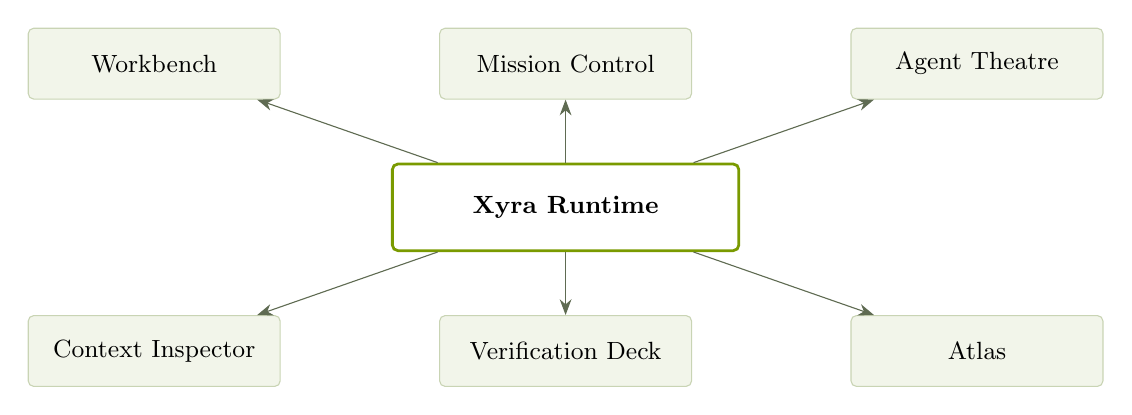
\begin{tikzpicture}[
  node distance=6mm,
  surf/.style={draw=xyraline,fill=xyrapanel,rounded corners=2pt,minimum height=9mm,minimum width=32mm,font=\small},
  core/.style={draw=xyralime,line width=1pt,fill=white,rounded corners=2pt,minimum height=11mm,minimum width=44mm,font=\small\bfseries}
]
\node[core] (rt) {Xyra Runtime};
\node[surf,above left=8mm and 14mm of rt] (wb) {Workbench};
\node[surf,above=8mm of rt] (mc) {Mission Control};
\node[surf,above right=8mm and 14mm of rt] (at) {Agent Theatre};
\node[surf,below left=8mm and 14mm of rt] (ci) {Context Inspector};
\node[surf,below=8mm of rt] (vd) {Verification Deck};
\node[surf,below right=8mm and 14mm of rt] (al) {Atlas};
\foreach \n in {wb,mc,at,ci,vd,al} \draw[xyragrey,-{Stealth[length=2mm]}] (rt) -- (\n);
\end{tikzpicture}
\caption{The runtime owns all state. Surfaces are projections of that state, never owners of it.}
\end{figure}

\section{Non goals}

Stating what Xyra does not attempt is as load bearing as stating what it does.

\begin{itemize}
  \item Xyra is not a general purpose text editor competing on startup time for editing a
  single configuration file. It is a project scale environment.
  \item Xyra does not host models. It orchestrates model providers the developer already
  pays for, including local ones.
  \item Xyra does not attempt to replace the shell or the browser. It drives them and reads
  their output.
  \item Xyra does not ship an interactive debugger in the first product generation. Runtime
  evidence reaches the agent through test output, traces and logs rather than through a
  breakpoint session, which is why no debug adapter appears in the issue register and no
  breakpoint control appears in the interface specification.
  \item Xyra does not implement its own version control. It drives git.
  \item Xyra does not implement real time collaborative editing. Multiple developers work
  through version control, and the collaboration surface in the title bar is reserved for a
  later generation.
  \item Xyra does not target mobile or web delivery in the first product generation.
\end{itemize}

The commercial model, pricing and edition split are deliberately outside the scope of this
document. Chapter~\ref{ch:foundation} establishes the licensing position that keeps every
commercial option open, which is the only part of that decision that constrains engineering.

\chapter{Open Source Foundation and Licensing}
\label{ch:foundation}

\section{The commercial constraint}

Every dependency in Xyra must satisfy one rule: it must permit distribution of a binary
whose corresponding source is not disclosed. In practice this means MIT, Apache~2.0, BSD,
ISC, Zlib, Unlicense or CC0. It excludes GPL and LGPL in linked form, and it excludes MPL~2.0
as well, for the reason given below.

This rule is what separates the standalone product from the current fork. It is not a
philosophical preference, it is the precondition for a commercial edition.

The allow list is exactly MIT, Apache-2.0, BSD-2-Clause, BSD-3-Clause, ISC, Zlib, Unlicense
and CC0-1.0. MPL-2.0 is \req{not} on it. Its copyleft is file scoped rather than project
scoped, which makes it survivable in principle, but a per file disclosure obligation inside a
commercial binary is a compliance burden with no compensating benefit when a permissive
alternative exists. A dependency outside the list enters only through an explicit entry in the
exception list inside the license check script, which puts the decision in front of a reviewer
rather than inside a transitive dependency nobody read.

\section{Verified license position}

The table below was compiled from the crates.io registry metadata and from the license
declarations inside each project, rather than from documentation or memory. Every entry was
checked while writing this document.

\begin{longtable}{@{}p{0.24\textwidth} p{0.30\textwidth} p{0.34\textwidth}@{}}
\toprule
\textbf{Component} & \textbf{License} & \textbf{Role in Xyra} \\
\midrule
\endfirsthead
\toprule
\textbf{Component} & \textbf{License} & \textbf{Role in Xyra} \\
\midrule
\endhead
\multicolumn{3}{@{}l}{\textit{Interface and rendering}}\\
gpui & Apache-2.0 & GPU accelerated UI framework, element tree, layout, input \\
wgpu & MIT OR Apache-2.0 & Graphics abstraction, fallback rendering path \\
vello & Apache-2.0 OR MIT & Vector rendering, alternative compositor path \\
cosmic-text & MIT OR Apache-2.0 & Text shaping and layout \\
swash & Apache-2.0 OR MIT & Font parsing, glyph rasterisation \\
\midrule
\multicolumn{3}{@{}l}{\textit{Editor core}}\\
ropey & MIT OR Apache-2.0 & Rope data structure for the text buffer \\
tree-sitter & MIT & Incremental parsing, concrete syntax trees \\
tree-sitter-highlight & MIT & Syntax highlighting over the parse tree \\
similar & Apache-2.0 & Text diffing for review surfaces \\
imara-diff & Apache-2.0 & High performance line diffing for large files \\
\midrule
\multicolumn{3}{@{}l}{\textit{Language intelligence}}\\
lsp-types & MIT & Language server protocol type definitions \\
tower-lsp or hand rolled client & MIT & Language server transport and lifecycle \\
\midrule
\multicolumn{3}{@{}l}{\textit{Project and system}}\\
gix (gitoxide) & MIT OR Apache-2.0 & Pure Rust git implementation \\
ignore & Unlicense OR MIT & Gitignore aware directory traversal \\
globset & Unlicense OR MIT & Glob matching for path rules \\
notify & CC0-1.0 & Filesystem watching \\
alacritty\_terminal & Apache-2.0 & Terminal emulation backend \\
tokio & MIT & Asynchronous runtime for the service layer \\
dashmap & MIT & Concurrent maps for shared indices \\
\midrule
\multicolumn{3}{@{}l}{\textit{Retrieval and storage}}\\
tantivy & MIT & Full text and structural search index \\
usearch & Apache-2.0 & Approximate nearest neighbour vector index \\
fastembed & Apache-2.0 & Local embedding generation \\
candle-core & MIT OR Apache-2.0 & Local model execution for embeddings and rerankers \\
tiktoken-rs & MIT & Token counting for budget accounting \\
redb & MIT OR Apache-2.0 & Embedded key value store for the durable state \\
rusqlite & MIT & Relational store for the graph and journal \\
zstd & MIT & Compression of context artefacts and caches \\
\midrule
\multicolumn{3}{@{}l}{\textit{Agent integration}}\\
agent-client-protocol & Apache-2.0 & Protocol for external agent processes \\
rmcp & Apache-2.0 & Model context protocol client and server \\
wasmtime & Apache-2.0 WITH LLVM-exception & Sandboxed extension execution \\
\midrule
\multicolumn{3}{@{}l}{\textit{Interface support}}\\
fuzzy-matcher & MIT & Fuzzy matching for pickers and the palette \\
\bottomrule
\caption{Verified license position of the proposed dependency set.}
\end{longtable}

\section{What this table means}

Two conclusions follow directly.

First, \req{a complete IDE can be assembled without touching a single copyleft dependency}.
The UI framework, the rope, the parser, the terminal, the git implementation, the language
server client, the vector index and the extension sandbox are all permissive. There is no
component in the critical path that forces source disclosure.

Second, \req{the highest leverage reuse is gpui}. It is Apache~2.0, it is production proven
in a shipping editor, and it solves the single hardest problem in this project, which is a
GPU accelerated UI framework with correct text rendering and input handling on three
platforms. Writing that from scratch would consume the majority of the engineering budget
and produce a worse result. Using it is not a compromise on independence, because Apache~2.0
imposes no disclosure obligation and no upstream coupling beyond the version we pin.

\section{Dependency strategy}

\begin{description}[style=nextline,leftmargin=0pt]
  \item[Vendor and pin the UI framework.] gpui is vendored into the repository at a pinned
  revision under its Apache~2.0 license with attribution preserved. Upstream changes are
  merged deliberately, never automatically. This removes the rebase treadmill that
  characterises the fork.

  \item[Wrap every third party boundary.] Editor code never calls gpui directly. It calls
  \ctl{xyra-ui}, a thin internal crate that re-exports the element model we actually use.
  The same applies to the parser, the git layer and the terminal. The cost is one indirection
  and the benefit is that any dependency can be replaced without touching product code.

  \item[Prefer boring dependencies.] Fewer, larger, well maintained crates over many small
  ones. Every dependency is a license question, a supply chain question and a maintenance
  question.

  \item[No network dependency at build time.] The build must succeed from a vendored source
  tree with no registry access, which is a hard requirement for reproducibility and for
  enterprise customers with air gapped environments.
\end{description}

\section{License hygiene in the repository}

\begin{itemize}
  \item A machine readable manifest at \ctl{licenses/manifest.toml} lists every dependency,
  its license, its source and the reason it is present.
  \item A continuous integration job fails the build when a dependency appears whose license
  is not on the allow list, using cargo-deny or an equivalent check.
  \item Vendored third party source lives under \ctl{third\_party/} with its original license
  file intact and unmodified.
  \item The notice file shipped with the product aggregates every attribution required by
  the Apache~2.0 and MIT terms.
\end{itemize}

\section{Reference implementations worth studying}

These projects are not dependencies. They are prior art whose architecture repays study
before writing the equivalent subsystem. All are permissively licensed, so reading them
carries no contamination risk, and porting an approach from them is legally clean when the
license is respected and attribution given.

\begin{table}[h]
\centering
\small
\begin{tabularx}{\textwidth}{l l X}
\toprule
\textbf{Project} & \textbf{License} & \textbf{What to learn from it} \\
\midrule
Helix & MPL-2.0 & Multi cursor and selection model, tree-sitter integration depth \\
Lapce & Apache-2.0 & Rope plus WASM plugin boundary, multi window process model \\
Zed gpui & Apache-2.0 & Element tree, layout engine, GPU text pipeline \\
Alacritty & Apache-2.0 & Terminal grid, escape sequence handling, performance discipline \\
Tantivy & MIT & Index segment design, query planning \\
Wasmtime & Apache-2.0 & Capability based sandboxing for untrusted extensions \\
Ripgrep and ignore & MIT & Directory traversal that respects ignore semantics at speed \\
\bottomrule
\end{tabularx}
\caption{Permissively licensed prior art.}
\end{table}

\chapter{System Architecture}
\label{ch:architecture}

\section{Layering}

Xyra is organised as five layers. Each layer may call downward and emit events upward. No
layer may call upward directly. This rule is what keeps the surfaces replaceable and the
core testable without a display.

\begin{figure}[h]
\centering
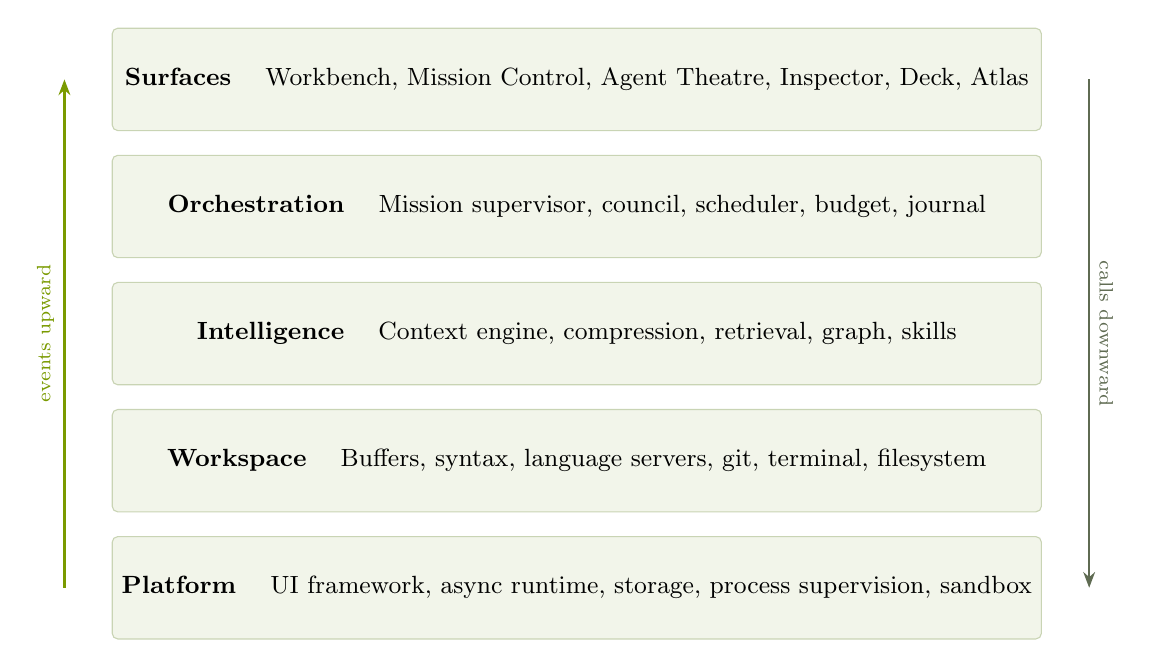
\begin{tikzpicture}[
  layer/.style={draw=xyraline,fill=xyrapanel,minimum width=118mm,minimum height=13mm,rounded corners=2pt,font=\small},
  lab/.style={font=\scriptsize\color{xyragrey}}
]
\node[layer] (l5) at (0,0) {\textbf{Surfaces} \quad Workbench, Mission Control, Agent Theatre, Inspector, Deck, Atlas};
\node[layer,below=3mm of l5] (l4) {\textbf{Orchestration} \quad Mission supervisor, council, scheduler, budget, journal};
\node[layer,below=3mm of l4] (l3) {\textbf{Intelligence} \quad Context engine, compression, retrieval, graph, skills};
\node[layer,below=3mm of l3] (l2) {\textbf{Workspace} \quad Buffers, syntax, language servers, git, terminal, filesystem};
\node[layer,below=3mm of l2] (l1) {\textbf{Platform} \quad UI framework, async runtime, storage, process supervision, sandbox};

\draw[-{Stealth[length=2mm]},xyralime,line width=0.8pt] ($(l1.west)+(-6mm,0)$) -- ($(l5.west)+(-6mm,0)$) node[midway,left,lab,rotate=90,anchor=south] {events upward};
\draw[-{Stealth[length=2mm]},xyragrey,line width=0.8pt] ($(l5.east)+(6mm,0)$) -- ($(l1.east)+(6mm,0)$) node[midway,right,lab,rotate=-90,anchor=south] {calls downward};
\end{tikzpicture}
\caption{Five layer architecture with a strict dependency direction.}
\end{figure}

\section{Process model}

Xyra runs as a small constellation of processes rather than one monolith. The reason is
containment: an agent process that hangs, a language server that leaks, or an extension that
panics must never take down the editor, and must never be able to block the interface
thread.

\begin{figure}[h]
\centering
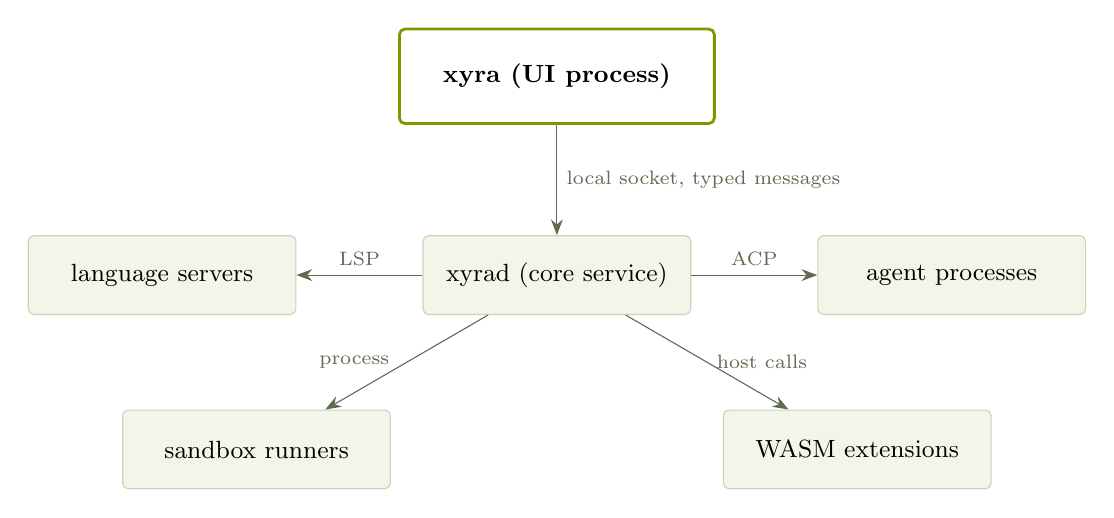
\begin{tikzpicture}[
  proc/.style={draw=xyraline,fill=xyrapanel,rounded corners=2pt,minimum height=10mm,minimum width=34mm,font=\small},
  main/.style={draw=xyralime,line width=1pt,fill=white,rounded corners=2pt,minimum height=12mm,minimum width=40mm,font=\small\bfseries},
  pipe/.style={-{Stealth[length=2mm]},xyragrey}
]
\node[main] (ui) at (0,0) {xyra (UI process)};
\node[proc,below=14mm of ui] (core) {xyrad (core service)};
\node[proc,left=16mm of core] (ls) {language servers};
\node[proc,right=16mm of core] (ag) {agent processes};
\node[proc,below left=12mm and 4mm of core] (sb) {sandbox runners};
\node[proc,below right=12mm and 4mm of core] (ext) {WASM extensions};

\draw[pipe] (ui) -- node[right,font=\scriptsize] {local socket, typed messages} (core);
\draw[pipe] (core) -- node[above,font=\scriptsize] {LSP} (ls);
\draw[pipe] (core) -- node[above,font=\scriptsize] {ACP} (ag);
\draw[pipe] (core) -- node[left,font=\scriptsize,xshift=-1mm] {process} (sb);
\draw[pipe] (core) -- node[right,font=\scriptsize] {host calls} (ext);
\end{tikzpicture}
\caption{Process topology. The interface never speaks to an agent or a language server directly.}
\end{figure}

\begin{description}[style=nextline,leftmargin=0pt]
  \item[xyra] The interface process. Owns the window, the element tree, input handling and
  rendering. Holds no authoritative state; it renders a projection pushed from the core and
  sends intents back.

  \item[xyrad] The core service. Owns buffers, the project model, the context engine, the
  mission supervisor, the journal and all persistence. Survives interface restarts, which
  means a crashed window never loses a running mission.

  \item[Language servers] One child per language per workspace, supervised with restart
  backoff and a health probe.

  \item[Agent processes] External agent binaries speaking the agent client protocol over
  stdio. Each runs in its own working directory with an environment the core constructs.

  \item[Sandbox runners] Ephemeral processes executing tests inside an isolated worktree.
  Killed on budget expiry without affecting anything else.

  \item[WASM extensions] Untrusted third party code with an explicit capability list, no
  ambient filesystem access and no network unless granted.
\end{description}

\section{Crate topology}

\begin{longtable}{@{}p{0.26\textwidth} p{0.66\textwidth}@{}}
\toprule
\textbf{Crate} & \textbf{Responsibility} \\
\midrule
\endfirsthead
\toprule
\textbf{Crate} & \textbf{Responsibility} \\
\midrule
\endhead
xyra-ui & Element model wrapper over the vendored UI framework, theme tokens, primitives \\
xyra-text & Rope buffer, transactions, undo history, multi cursor selection algebra \\
xyra-syntax & Parser host, incremental reparse, highlight queries, structural selection \\
xyra-lang & Language server client, capability negotiation, diagnostics, completion \\
xyra-project & Worktree model, ignore semantics, file watching, path resolution \\
xyra-vcs & Git operations, status, diff, blame, staging, commit, branch \\
xyra-term & Terminal grid, PTY supervision, escape parsing, search \\
xyra-context & Symbol and import graph, retrieval, compression pipeline, budget solver \\
xyra-memory & Durable stores, caches, journal, mission state, migrations \\
xyra-agent & Agent process supervision, protocol clients, tool exposure, transcript capture \\
xyra-mission & Ticket graph, supervisor loop, failure policy, budgets \\
xyra-verify & Sandbox execution, visual verification, quality assurance sweeps, flags \\
xyra-fleet & Multi repository registry, cross repository search and impact \\
xyra-skills & Skill registry, resolution, injection, precedence \\
xyra-ext & Extension host, capability enforcement, manifest validation \\
xyra-proto & Message types shared between the interface and the core \\
xyrad & Core service binary, wiring, supervision tree \\
xyra & Interface binary, surfaces, keymap, command registry \\
\bottomrule
\caption{Crate responsibilities. One crate, one reason to change.}
\end{longtable}

\section{State ownership and the projection model}

The interface holds no authoritative state. Every surface receives a projection: a
serialisable snapshot of exactly what it needs to render, versioned so that stale frames are
discarded. User actions travel back as intents, never as mutations.

\begin{figure}[h]
\centering
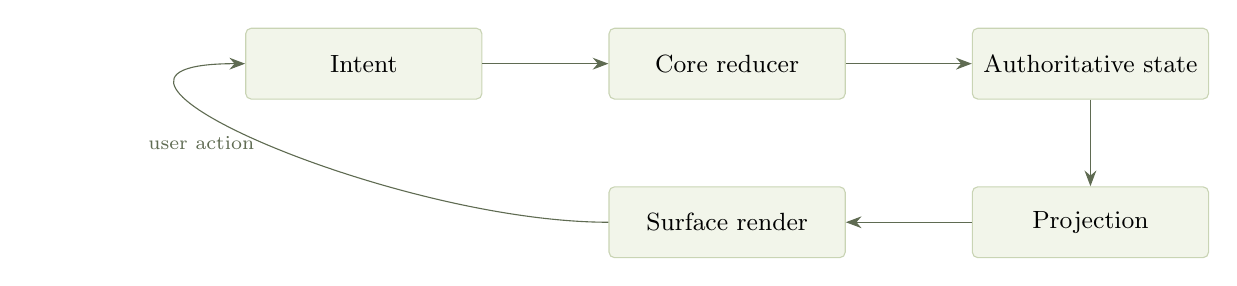
\begin{tikzpicture}[
  box/.style={draw=xyraline,fill=xyrapanel,rounded corners=2pt,minimum height=9mm,minimum width=30mm,font=\small},
  arr/.style={-{Stealth[length=2mm]},xyragrey}
]
\node[box] (intent) {Intent};
\node[box,right=16mm of intent] (core) {Core reducer};
\node[box,right=16mm of core] (state) {Authoritative state};
\node[box,below=11mm of state] (proj) {Projection};
\node[box,left=16mm of proj] (surface) {Surface render};

\draw[arr] (intent) -- (core);
\draw[arr] (core) -- (state);
\draw[arr] (state) -- (proj);
\draw[arr] (proj) -- (surface);
\draw[arr] (surface) to[out=180,in=180,looseness=1.4] node[left,font=\scriptsize] {user action} (intent);
\end{tikzpicture}
\caption{Unidirectional flow. The loop is closed only by user action.}
\end{figure}

This is what makes the product testable. Every surface can be exercised by feeding
projections and asserting on the intents produced, with no window open and no GPU present.

\section{Concurrency model}

\begin{itemize}
  \item The interface thread never blocks. Any operation with unbounded duration is a task
  on the core's runtime, and the interface shows an intermediate state.
  \item Buffer edits are applied on a single owning task per buffer. Concurrent edits arrive
  as transactions and are ordered, never merged optimistically.
  \item Indexing, embedding and graph construction run on a bounded worker pool sized to
  physical cores minus two, so the machine stays usable.
  \item Every long running task carries a cancellation token and a budget. A task without a
  budget is a defect.
  \item Agent sessions are supervised with a timeout, an inactivity watchdog and a hard kill
  path, because the dominant real world failure is a subprocess that never exits.
\end{itemize}

\section{Persistence}

\begin{table}[h]
\centering
\small
\begin{tabularx}{\textwidth}{l l X}
\toprule
\textbf{Store} & \textbf{Technology} & \textbf{Contents} \\
\midrule
Project index & SQLite & Symbols, import edges, file hashes, chunk metadata \\
Vector index & Embedded ANN file & Chunk embeddings, quantised, memory mapped \\
Mission state & JSON with atomic replace & Ticket graph, attempts, budgets, commits \\
Journal & Append only JSON lines & Decisions, verdicts, verification results \\
Caches & Content addressed files & Compression artefacts, screenshots, transcripts \\
Settings & TOML & User and workspace configuration, layered \\
\bottomrule
\end{tabularx}
\caption{Storage responsibilities. Nothing important lives only in memory.}
\end{table}

Every store is per workspace under \ctl{.xyra/} except global caches, which live under the
platform cache directory. Deleting \ctl{.xyra/} must degrade the product to a cold start and
never corrupt the repository.

\section{Failure containment}

\begin{longtable}{@{}p{0.30\textwidth} p{0.62\textwidth}@{}}
\toprule
\textbf{Failure} & \textbf{Containment} \\
\midrule
\endhead
Language server crash & Supervised restart with exponential backoff, diagnostics preserved, editing unaffected \\
Agent process hang & Inactivity watchdog kills the session, ticket is marked failed, supervisor continues \\
Extension panic & WASM trap is caught, extension is disabled for the session, a flag is raised \\
Core service crash & Interface shows a reconnect state, mission resumes from durable state on restart \\
Interface crash & Core keeps working, mission continues, window reopens onto live state \\
Disk full & Writes fail closed, mission halts with a stated reason, nothing is half written \\
Corrupt index & Detected by checksum, index rebuilt in background, structural queries degrade to search \\
\bottomrule
\caption{Every failure has a named containment strategy.}
\end{longtable}

\chapter{The Context Engine}
\label{ch:context}

\section{The objective function}

Every agentic editor faces the same problem and almost none of them state it as an
optimisation. Given a token budget $B$, choose a set of context items $S$ that maximises the
probability the agent produces a correct action.

\[
\max_{S} \; P(\text{correct action} \mid S) \quad \text{subject to} \quad \sum_{i \in S} \text{tokens}(i) \le B
\]

The naive implementation ranks chunks by embedding similarity and fills the budget until it
overflows. This is wrong in three distinct ways. It ignores that some items are load bearing
regardless of similarity, such as the exact signature of the function being modified. It
ignores that many high similarity items are redundant with each other. And it pays full
token price for information that could be represented at a fraction of the cost without
losing decision value.

Xyra treats this as a compression problem with a value model. The engine is built from four
mechanisms: structural representation, tiered escalation, delta encoding, and a budget
solver. Around them sit accelerators that reduce latency and cost without changing the
selected set.

\section{Structural Context Protocol}

The Structural Context Protocol, abbreviated SCP, is the canonical representation of a source
file inside Xyra. It is not the file text. It is a projection of the file's parse tree into a
form that preserves everything an agent needs to reason about the file's interface and
dependencies, while discarding the bodies it does not need.

An SCP record for a file contains the module path and language, the ordered list of exported
and internal symbols with their full signatures, type declarations in full, documentation
comments attached to symbols, the import list resolved to concrete paths, the outbound call
edges by symbol, and a stable content hash per symbol body so a body can be requested later
by handle.

\begin{table}[h]
\centering
\small
\begin{tabularx}{\textwidth}{l r r X}
\toprule
\textbf{Representation} & \textbf{Tokens} & \textbf{Ratio} & \textbf{Preserves} \\
\midrule
Raw file text & 3200 & 1.00 & Everything \\
SCP level 2 & 980 & 0.31 & Signatures, types, docs, imports, call edges, body handles \\
SCP level 1 & 420 & 0.13 & Signatures, types, imports \\
SCP level 0 & 130 & 0.04 & Module path, exported symbol names, import list \\
\bottomrule
\end{tabularx}
\caption{Indicative compression profile for a typical eight hundred line source file. Ratios are
representative of the design target, and the harness in Chapter~\ref{ch:quality} measures the
real distribution per language.}
\end{table}

The critical property is that SCP is \req{lossless with respect to the interface}. An agent
reading SCP level 2 knows every symbol it can call, with exact parameter types and return
types. It does not know how those symbols are implemented, and in the majority of tasks it
does not need to. When it does, it asks.

\section{Tiered escalation}

Context is assembled as a ladder, and the agent climbs it only where it must. This inverts
the usual flow, in which the editor guesses what the agent needs before the agent has
reasoned about the task.

\begin{figure}[h]
\centering
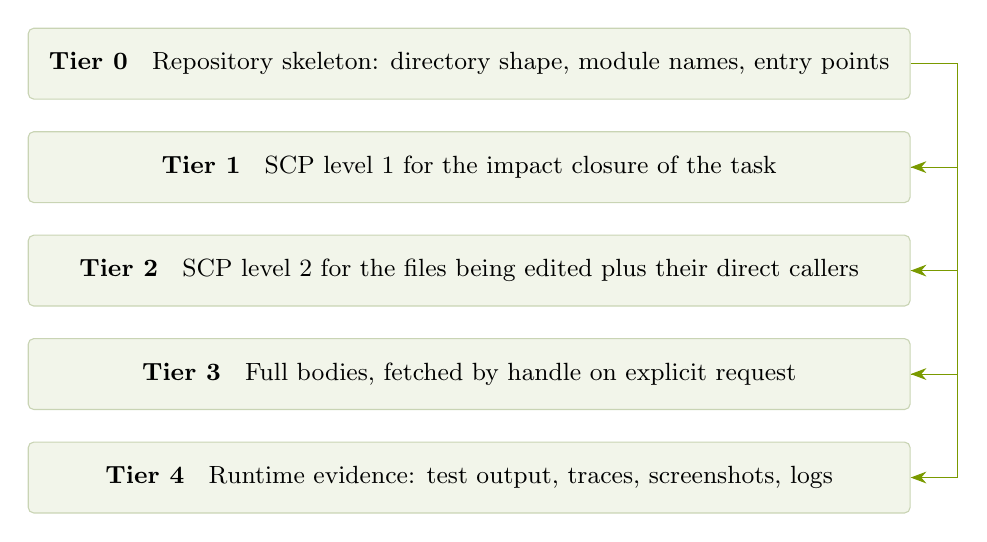
\begin{tikzpicture}[
  tier/.style={draw=xyraline,fill=xyrapanel,rounded corners=2pt,minimum height=9mm,minimum width=112mm,font=\small},
  arr/.style={-{Stealth[length=2mm]},xyralime}
]
\node[tier] (t0) at (0,0) {\textbf{Tier 0} \; Repository skeleton: directory shape, module names, entry points};
\node[tier,below=4mm of t0] (t1) {\textbf{Tier 1} \; SCP level 1 for the impact closure of the task};
\node[tier,below=4mm of t1] (t2) {\textbf{Tier 2} \; SCP level 2 for the files being edited plus their direct callers};
\node[tier,below=4mm of t2] (t3) {\textbf{Tier 3} \; Full bodies, fetched by handle on explicit request};
\node[tier,below=4mm of t3] (t4) {\textbf{Tier 4} \; Runtime evidence: test output, traces, screenshots, logs};
\draw[arr] (t0.east) -- ++(6mm,0) |- (t1.east);
\draw[arr] (t1.east) -- ++(6mm,0) |- (t2.east);
\draw[arr] (t2.east) -- ++(6mm,0) |- (t3.east);
\draw[arr] (t3.east) -- ++(6mm,0) |- (t4.east);
\end{tikzpicture}
\caption{The context ladder. Escalation is driven by the agent's own tool calls, not by
the editor's guess.}
\end{figure}

Tier~0 and Tier~1 are pushed into the session automatically because they are cheap and
always relevant. Tier~2 is computed from the deterministic impact closure described in
Section~\ref{sec:structural}. Tier~3 and Tier~4 are pulled by the agent through tools, which
means the cost is paid only when the information is actually wanted.

\section{Structural retrieval}
\label{sec:structural}

Before any embedding is consulted, Xyra answers the question structurally.

\begin{description}[style=nextline,leftmargin=0pt]
  \item[Import graph.] Parsed from source, resolved to concrete files, stored as edges. Gives
  the exact set of files that would break if a module changes, by transitive distance.
  \item[Symbol table.] Every definition with its kind, location and visibility, so a symbol
  name resolves to a definition without similarity search.
  \item[Call edges.] Outbound calls per symbol, which produces a call closure for a change to
  a single function rather than a whole file.
  \item[Test mapping.] Which test files exercise which source files, derived from imports and
  from execution traces when available. This makes the verification loop targeted rather than
  running the whole suite each time.
  \item[Blame and history.] Which commits last touched the region, which gives an agent the
  reason a line exists before it deletes it.
\end{description}

Embedding search is consulted for a narrow class of questions: locating behaviour described
in prose when the developer does not know the symbol name. It is a fallback, and the
interface labels its results as such so the developer can see when the machine is guessing.

\section{Semantic delta encoding}

Within a mission, consecutive sessions overlap heavily. Re-sending the same skeleton on every
ticket wastes a large fraction of the budget. Xyra addresses this with a delta protocol.

The core maintains, per mission, a content addressed dictionary of context items already
transmitted. When assembling the next session, items already in the dictionary are referenced
by handle rather than repeated, and the session preamble carries only the delta: what changed
since the last transmission, plus the handles for everything unchanged.

\begin{table}[h]
\centering
\small
\begin{tabularx}{\textwidth}{l X r}
\toprule
\textbf{Element} & \textbf{Encoding} & \textbf{Cost} \\
\midrule
Unchanged file, previously sent & Handle reference with symbol list & Tens of tokens \\
Changed file & Delta against the previous SCP record & Proportional to the change \\
New file in scope & Full SCP record at the required tier & Full record cost \\
Removed from scope & Explicit eviction notice & Negligible \\
\bottomrule
\end{tabularx}
\caption{Delta encoding between sessions in a mission.}
\end{table}

Because each ticket runs in a fresh session, the dictionary is not a context window trick. It
is a compact resumption record that lets a new session reach the same understanding as its
predecessor for a fraction of the tokens.

\section{The budget solver}

Given candidate items with an estimated value and a measured token cost, selection is a
knapsack problem with dependencies and redundancy penalties.

\begin{itemize}
  \item \req{Value} combines structural proximity to the task target, recency of change,
  authorship of the failing test, and explicit developer pinning. Similarity contributes, but
  it never dominates a structural signal.
  \item \req{Cost} is measured with a real tokeniser for the target model, not estimated by
  character count. Estimating by characters is wrong by up to forty percent on code.
  \item \req{Redundancy} is penalised. Two chunks with near identical content contribute once.
  \item \req{Dependencies} are respected. Including a symbol implies including the types in
  its signature.
  \item \req{Floors} are enforced. The file being edited is always at Tier~2 regardless of the
  solver's opinion, because omitting it produces confident nonsense.
\end{itemize}

The solver runs greedily by value density with a repair pass, which is fast enough to run on
every assembly and close enough to optimal that the difference does not matter in practice.

\section{Accelerators}

Compression reduces cost. Accelerators reduce latency and repeated work. They do not change
which items are selected, which keeps them safe to enable by default.

\begin{longtable}{@{}p{0.28\textwidth} p{0.64\textwidth}@{}}
\toprule
\textbf{Accelerator} & \textbf{Mechanism} \\
\midrule
\endhead
Stable prefix ordering & Context is emitted in a canonical order with the invariant material
first, so provider side prefix caches hit across sessions instead of missing on reordering. \\
Speculative prefetch & While the agent is reasoning, the graph predicts the next files it
will request and warms their SCP records and bodies. \\
Incremental embedding & Content hashed per chunk, so only changed chunks are re-embedded.
A file rename costs nothing. \\
Quantised vector index & Embeddings stored quantised and memory mapped, which keeps a large
repository index resident without dominating memory. \\
Local reranking & A small cross encoder run locally reorders the candidate set before the
budget solver, which improves selection quality without a network call. \\
Parallel lens execution & Independent review lenses run concurrently rather than in
sequence, so an adversarial review costs one lens of latency rather than three. \\
Warm sandbox worktrees & A pool of prepared worktrees with dependencies already installed,
so verification does not pay the setup cost on every ticket. \\
Test selection & The test mapping restricts verification to the tests that can be affected,
with a full suite run at ticket boundaries and before completion. \\
Streaming to disk & Agent output is persisted as it arrives, so a crashed session is
resumable and a long transcript never lives only in memory. \\
Compression of artefacts & Transcripts, screenshots and traces are stored compressed and
content addressed, deduplicated across missions. \\
\bottomrule
\caption{Latency and cost accelerators.}
\end{longtable}

\section{Context expansion integrations}

Structural knowledge of the repository is necessary but not sufficient. A large class of
agent errors comes from information that simply is not in the code. These integrations bring
that information into the ladder as first class context, each behind an explicit capability
so a developer can see and control what leaves the machine.

\begin{longtable}{@{}p{0.26\textwidth} p{0.30\textwidth} p{0.36\textwidth}@{}}
\toprule
\textbf{Integration} & \textbf{Brings in} & \textbf{Answers the question} \\
\midrule
\endhead
Language server & Hover types, call hierarchy, references, definitions & What is the real type here, who calls this \\
Version history & Blame, commit messages, pull request bodies & Why does this line exist \\
Issue tracker & Linked issues, acceptance criteria & What was actually asked for \\
Documentation fetch & Current library documentation by version & What is the correct API today, not at training time \\
Runtime traces & Execution paths, values at failure & What actually happened, not what should have \\
Test results & Failure output, flake history & Which failures are real \\
Design assets & Exported mockups, design tokens & What is this supposed to look like \\
Schema and migrations & Database schema, pending migrations & What shape is the data \\
Observability & Error rates, slow queries, recent incidents & What is breaking in production \\
Dependency registry & Package sizes, versions, advisories & What does adding this cost \\
Fleet siblings & Contracts consumed by other repositories & Who else breaks if this changes \\
Terminal history & Recent commands and their output & What has the developer already tried \\
\bottomrule
\caption{Context expansion integrations and the question each one closes.}
\end{longtable}

\section{The assembly pipeline}

\begin{figure}[h]
\centering
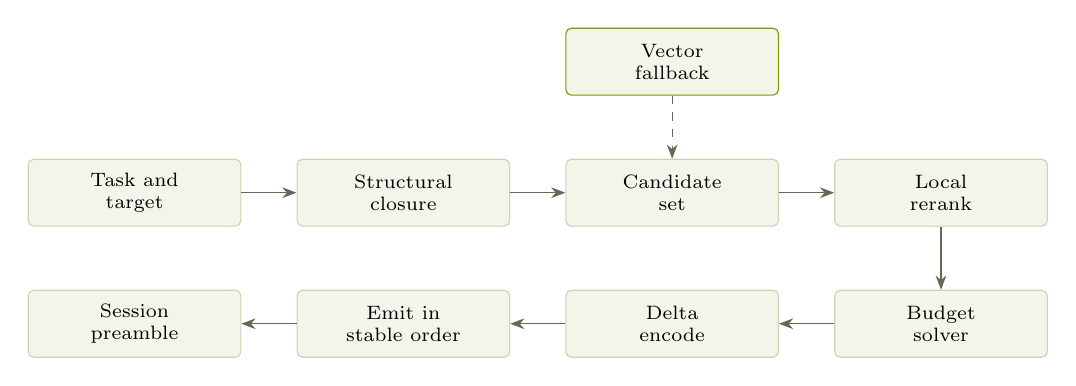
\begin{tikzpicture}[
  st/.style={draw=xyraline,fill=xyrapanel,rounded corners=2pt,minimum height=8.5mm,minimum width=27mm,font=\scriptsize,align=center},
  arr/.style={-{Stealth[length=1.8mm]},xyragrey}
]
\node[st] (task) {Task and\\target};
\node[st,right=7mm of task] (struct) {Structural\\closure};
\node[st,right=7mm of struct] (cand) {Candidate\\set};
\node[st,right=7mm of cand] (rank) {Local\\rerank};
\node[st,below=8mm of rank] (solve) {Budget\\solver};
\node[st,left=7mm of solve] (delta) {Delta\\encode};
\node[st,left=7mm of delta] (emit) {Emit in\\stable order};
\node[st,left=7mm of emit] (sess) {Session\\preamble};

\draw[arr] (task) -- (struct);
\draw[arr] (struct) -- (cand);
\draw[arr] (cand) -- (rank);
\draw[arr] (rank) -- (solve);
\draw[arr] (solve) -- (delta);
\draw[arr] (delta) -- (emit);
\draw[arr] (emit) -- (sess);

\node[st,above=8mm of cand,draw=xyralime] (vec) {Vector\\fallback};
\draw[arr,dashed] (vec) -- (cand);
\end{tikzpicture}
\caption{Context assembly. Similarity search enters only as a labelled fallback.}
\end{figure}

\section{Measurement}

None of this is worth shipping unless it is measured. The context engine carries a permanent
evaluation harness with four metrics, reported per mission and visible in the Context
Inspector.

\begin{itemize}
  \item \req{Budget utilisation.} Tokens spent versus tokens available, and the fraction
  spent on each tier.
  \item \req{Compression ratio.} Tokens emitted versus tokens the naive representation would
  have required for the same item set.
  \item \req{Escalation rate.} How often the agent had to climb to Tier~3, which is the
  signal that the lower tiers are under specified.
  \item \req{First attempt success.} The fraction of tickets whose first session passes
  verification, which is the only end to end measure that matters.
\end{itemize}

\chapter{The Agent Layer}
\label{ch:agents}

\section{Roles rather than one assistant}

A single general assistant is the wrong abstraction for autonomous work, because the
prompting, the tool set and the failure handling that make an implementer effective make a
reviewer credulous. Xyra runs a team of specialised roles with distinct mandates and distinct
tool grants.

\begin{table}[h]
\centering
\small
\begin{tabularx}{\textwidth}{l X l}
\toprule
\textbf{Role} & \textbf{Mandate} & \textbf{Write access} \\
\midrule
Planner & Decompose an objective into a dependency ordered ticket graph & None \\
Architect & Produce and defend a design, challenge another design & None \\
Implementer & Complete exactly one ticket, leave tests passing & Worktree \\
Reviewer & Cross examine a diff through one lens, return a structured verdict & None \\
Verifier & Execute tests, render pages, run quality sweeps, report facts & Sandbox only \\
Repairer & Fix a specific named failure inside a snapshot & Snapshot \\
Replanner & Split a repeatedly failing ticket into smaller tickets & None \\
Scribe & Summarise, journal, produce release notes and reports & Documents \\
\bottomrule
\end{tabularx}
\caption{Agent roles. Write access is a property of the role, not of the model.}
\label{tab:roles}
\end{table}

Visual verification, quality sweeps and cross repository analysis are capabilities of the
Verifier role rather than separate roles, which keeps the role set closed at eight. The Agent
Theatre in Chapter~\ref{ch:interface} renders exactly one lane per role in this table.

The vendor behind each role is configurable, and the default deliberately places the reviewer
on a different vendor from the implementer. A model reviewing its own output shares its own
blind spots.

\section{The mission supervisor}

The supervisor is the component that makes unattended work possible. It owns a durable ticket
graph and drives it to completion without asking the developer anything it can resolve
itself.

\begin{figure}[h]
\centering
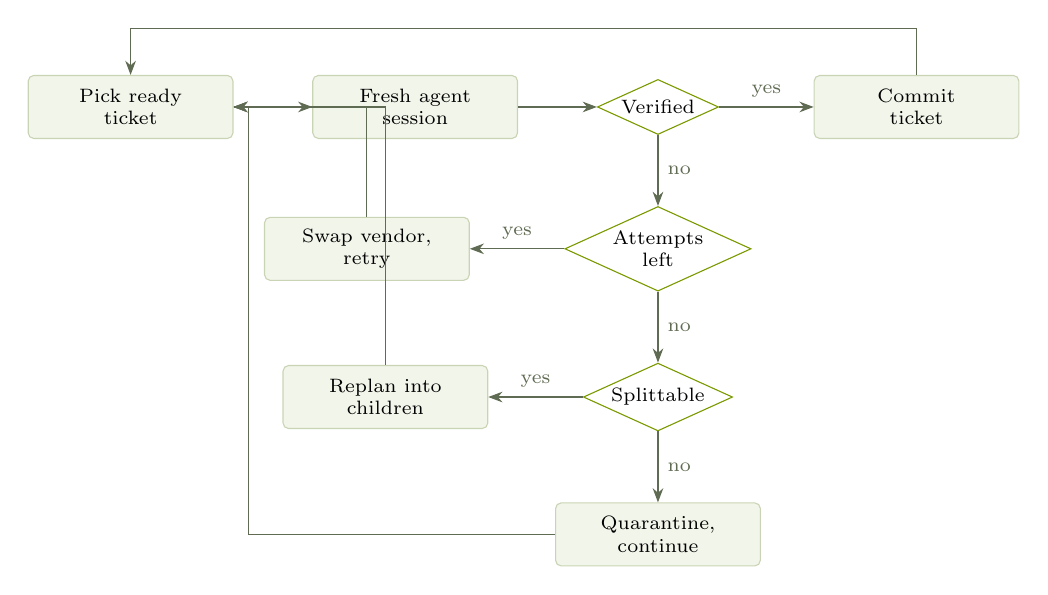
\begin{tikzpicture}[
  st/.style={draw=xyraline,fill=xyrapanel,rounded corners=2pt,minimum height=8mm,minimum width=26mm,font=\scriptsize,align=center},
  dec/.style={draw=xyralime,fill=white,diamond,aspect=2.2,inner sep=1pt,font=\scriptsize,align=center},
  arr/.style={-{Stealth[length=1.8mm]},xyragrey,font=\scriptsize}
]
\node[st] (pick) {Pick ready\\ticket};
\node[st,right=10mm of pick] (run) {Fresh agent\\session};
\node[dec,right=10mm of run] (ver) {Verified};
\node[st,right=12mm of ver] (commit) {Commit\\ticket};
\node[dec,below=9mm of ver] (att) {Attempts\\left};
\node[st,left=12mm of att] (swap) {Swap vendor,\\retry};
\node[dec,below=9mm of att] (split) {Splittable};
\node[st,left=12mm of split] (children) {Replan into\\children};
\node[st,below=9mm of split] (quar) {Quarantine,\\continue};

\draw[arr] (pick) -- (run);
\draw[arr] (run) -- (ver);
\draw[arr] (ver) -- node[above] {yes} (commit);
\draw[arr] (ver) -- node[right] {no} (att);
\draw[arr] (att) -- node[above] {yes} (swap);
\draw[arr] (att) -- node[right] {no} (split);
\draw[arr] (split) -- node[above] {yes} (children);
\draw[arr] (split) -- node[right] {no} (quar);
\draw[arr] (swap) |- (pick);
\draw[arr] (children) |- (pick);
\draw[arr] (commit) |- ++(0,10mm) -| (pick);
\draw[arr] (quar) -| ++(-52mm,0) |- (pick);
\end{tikzpicture}
\caption{Supervisor loop. Failure is a policy with four escalations, never a stop.}
\end{figure}

\subsection{Why fresh sessions}

The central design decision is that each ticket runs in a session that has never seen any
other ticket. This is counterintuitive until the arithmetic is done. A session that
accumulates context degrades in two ways: it fills the window, and it accumulates the
residue of earlier reasoning, including earlier mistakes. A fresh session with a precise
brief and a compressed structural context reaches higher first attempt success than a long
running session at ticket fifty, and the total work a mission can perform stops being bounded
by any window at all.

\subsection{Durability}

Mission state is written atomically after every state transition. The consequences are
concrete: closing the laptop pauses a mission, a crash loses at most the ticket in flight,
and resuming is a single command that reads the graph and continues. The state file is the
mission; the process is disposable.

\subsection{Budgets and brakes}

Autonomy without limits is a liability. Every mission carries hard caps on total sessions,
wall clock duration, attempts per ticket and consecutive failures, plus a stop flag the
developer can set at any moment which halts the loop after the ticket in flight completes.
Exceeding any cap halts the mission with a stated reason rather than continuing on hope.

\section{Verification}

\subsection{Isolated execution}

Verification never runs in the developer's working tree. The supervisor snapshots the
uncommitted change set into a throwaway worktree and executes the project's own test or build
command there. The developer's tree is untouched, which means verification can run while the
developer keeps working, and a failed attempt cannot leave debris behind.

\subsection{Visual verification}

For any change with a reachable page, a verifier renders it headless, captures a screenshot
and asks a vision capable model whether the result matches the stated intent. The verdict is
structured, with issues ranked by severity, which is what makes it usable inside an automatic
fix loop rather than as decoration. A design export can be supplied, in which case the
comparison is against the intended design rather than against a description.

\subsection{Adversarial review}

The council runs a diff past a rival vendor through independent lenses, by default
correctness, security and house conventions, executed in parallel. Each lens returns findings
with severity, and a policy decides whether the aggregate blocks. Policy is per repository and
per path, so code that touches money or credentials can demand more lenses and block on lower
severities than code that touches a marketing page.

\subsection{Quality assurance sweeps}

A verifier drives the running application as a hostile user: crawling same origin pages,
filling every input with type aware adversarial values, clicking aggressively, and collecting
console errors, uncaught exceptions, server errors, failed requests, accessibility problems
and load timings. Findings are deduplicated and ranked, then fed back as tickets rather than
delivered as a raw log.

\section{Skills}

Skills are the mechanism by which a team encodes its own standards so that every agent
session inherits them without being told.

\begin{table}[h]
\centering
\small
\begin{tabularx}{\textwidth}{l X}
\toprule
\textbf{Skill} & \textbf{Encodes} \\
\midrule
Autonomy & Prove before presenting: verify, look at the result, analyse impact before touching shared contracts \\
Terminal discipline & Never run an interactive command or a process that does not exit, per tool flags tabulated \\
Conventions & House rules for code, commits and interface copy \\
Review & The checklist a reviewer applies, including domain specific traps \\
Domain safety & Rules for money arithmetic, credentials, and any high consequence domain \\
Shipping & The gate before a change leaves the machine \\
Prompt discipline & Turning a vague instruction into a scoped one before acting \\
\bottomrule
\end{tabularx}
\caption{The default skill set. Teams add their own.}
\end{table}

Skills resolve in a precedence chain: workspace, then user, then bundled defaults. A workspace
skill overrides a user skill of the same name, which lets a team enforce a standard on a
repository without touching anyone's personal configuration. The Context Inspector shows
exactly which skills were injected into any given session, because an invisible instruction
that changes behaviour is a debugging nightmare.

\section{Fleet operations}

A contract rarely lives in one repository. Fleet raises every structural capability from the
repository to the group.

\begin{itemize}
  \item Repositories are registered from the developer's version control provider, not from a
  hand written file, and missing ones are cloned on registration.
  \item Cross repository search resolves a symbol or endpoint name across every member.
  \item Cross repository impact separates the repository that defines a contract from those
  that consume it, and orders the resulting work accordingly.
  \item A fleet refactor executes the same intent through every affected repository in
  dependency order, verifying each one independently and preparing linked changes.
\end{itemize}

\section{Tool surface exposed to agents}

Agents act through a bounded tool set. Every tool is auditable, every tool is capability
gated, and no tool grants ambient authority.

\begin{longtable}{@{}p{0.24\textwidth} p{0.68\textwidth}@{}}
\toprule
\textbf{Tool} & \textbf{Contract} \\
\midrule
\endhead
read\_file & Returns a file at a requested SCP tier or in full, by handle \\
search\_code & Structural search first, similarity fallback clearly labelled \\
impact & Deterministic closure for a symbol or file, by transitive distance \\
graph & Neighbourhood of a file: imports, importers, defined symbols \\
edit & Applies a transaction to a buffer, always reversible \\
run\_tests & Executes the project's test command inside a snapshot \\
verify\_patch & Full verification of the current change set, returns a verdict \\
render\_check & Renders a page and returns a structured visual verdict \\
compare\_design & Renders a page and compares it against a design export \\
qa\_sweep & Drives the running application adversarially, returns ranked defects \\
fleet\_search & Cross repository search \\
fleet\_impact & Cross repository impact analysis \\
journal & Records a decision with its rationale against the current commit \\
ask\_developer & Escalates a genuine decision as a structured choice with costs \\
\bottomrule
\caption{Agent tool surface. Anything not on this list is not reachable.}
\end{longtable}

\section{Escalation to the developer}

The supervisor escalates only when a decision genuinely belongs to the human: an
architectural fork with real trade offs, an ambiguity in the objective that changes the
outcome, or an action with consequences outside the repository. Escalation is never a
terminal question. It is a structured choice: each option carries its measured cost, its
dependency weight and a sketch of the resulting structure, and the mission continues on
unblocked tickets while the choice is pending.

\chapter{Interface Specification}
\label{ch:interface}

This chapter specifies every surface, every region and every control. Each control carries a
stable identifier used by the implementation, the automated interface tests and the
accessibility layer. A control that is not in this chapter does not ship.

\section{Design system}

\subsection{Tokens}

\begin{table}[h]
\centering
\small
\begin{tabularx}{\textwidth}{l l X}
\toprule
\textbf{Token} & \textbf{Value} & \textbf{Applied to} \\
\midrule
space.1 to space.8 & 2, 4, 6, 8, 12, 16, 24, 32 & All padding and gaps, no arbitrary values \\
radius.sm / md / lg & 4, 6, 10 & Controls, cards, panels \\
control.height.sm & 28 & Compact toolbar controls \\
control.height.md & 34 & Default buttons, inputs \\
control.height.lg & 42 & Primary actions, empty state actions \\
text.xs to text.xl & 11, 12, 13, 15, 19 & Labels, body, headings \\
icon.sm / md / lg & 14, 16, 20 & Inline, control, feature \\
elevation.0 to 3 & Flat, subtle, raised, floating & Panels, popovers, dialogs, drag \\
\bottomrule
\end{tabularx}
\caption{Design tokens. Sizes are in logical pixels at a scale factor of one.}
\end{table}

\subsection{Rules that are not negotiable}

\begin{itemize}
  \item Every control carries a visible text label unless it is in a dense toolbar, and even
  then it carries an accessible name and a tooltip. Icon only interfaces are a discoverability
  failure.
  \item Minimum interactive target is thirty four logical pixels in the primary flow.
  \item Sentence case everywhere. No capitalised words in interface copy.
  \item Every destructive action is either reversible or confirmed, never both silent and
  permanent.
  \item Every long running action shows determinate progress when a total is known, and an
  elapsed counter when it is not.
  \item Colour never carries meaning alone. Severity is colour plus a glyph plus a word.
\end{itemize}

\section{Window anatomy}

\begin{figure}[h]
\centering
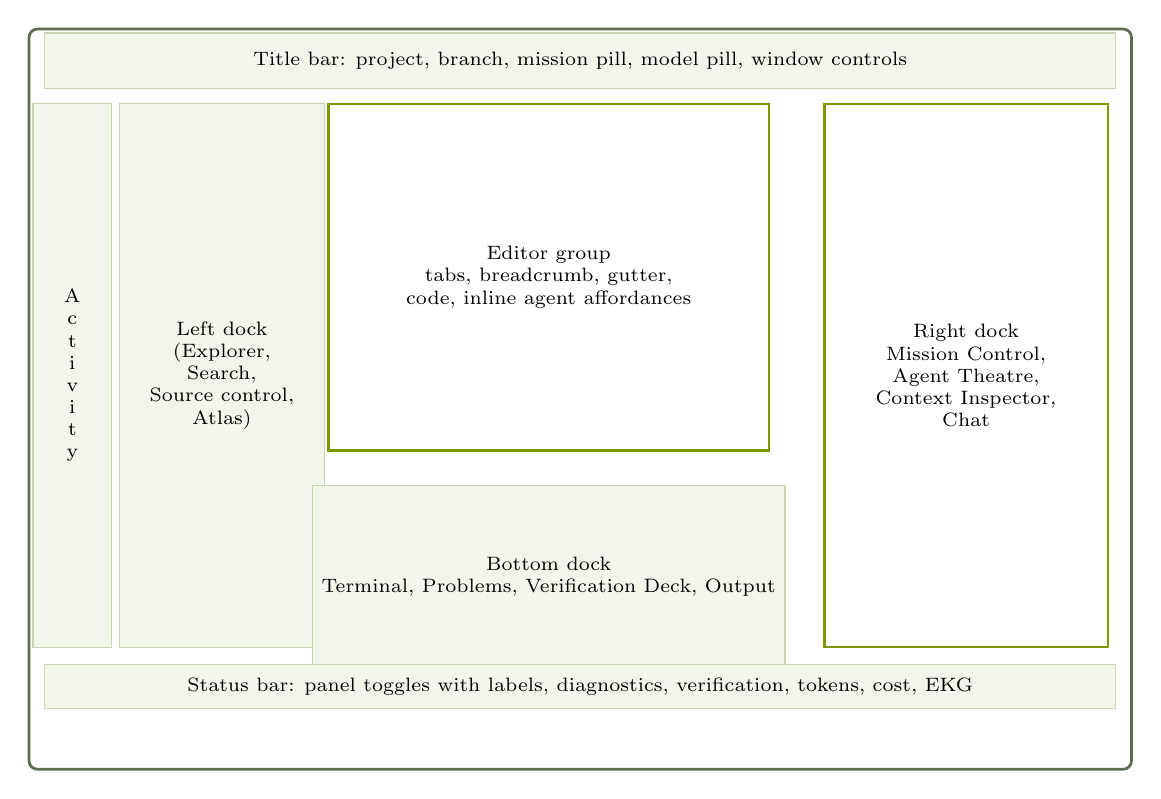
\begin{tikzpicture}[
  reg/.style={draw=xyraline,fill=xyrapanel,font=\scriptsize,align=center},
  hi/.style={draw=xyralime,line width=0.9pt,fill=white,font=\scriptsize,align=center}
]
\draw[draw=xyragrey,line width=1pt,rounded corners=3pt] (0,0) rectangle (14,9.4);
\node[reg,minimum width=13.6cm,minimum height=0.7cm] at (7,9.0) {Title bar: project, branch, mission pill, model pill, window controls};
\node[reg,minimum width=1.0cm,minimum height=6.9cm] at (0.55,5.0) {A\\c\\t\\i\\v\\i\\t\\y};
\node[reg,minimum width=2.6cm,minimum height=6.9cm] at (2.45,5.0) {Left dock\\(Explorer,\\Search,\\Source control,\\Atlas)};
\node[hi,minimum width=5.6cm,minimum height=4.4cm] at (6.6,6.25) {Editor group\\tabs, breadcrumb, gutter,\\code, inline agent affordances};
\node[reg,minimum width=5.6cm,minimum height=2.3cm] at (6.6,2.45) {Bottom dock\\Terminal, Problems, Verification Deck, Output};
\node[hi,minimum width=3.6cm,minimum height=6.9cm] at (11.9,5.0) {Right dock\\Mission Control,\\Agent Theatre,\\Context Inspector,\\Chat};
\node[reg,minimum width=13.6cm,minimum height=0.55cm] at (7,1.05) {Status bar: panel toggles with labels, diagnostics, verification, tokens, cost, EKG};
\end{tikzpicture}
\caption{Window regions. The right dock is where autonomous work is observed and steered.}
\end{figure}

\section{Title bar}

\begin{longtable}{@{}p{0.30\textwidth} p{0.24\textwidth} p{0.36\textwidth}@{}}
\toprule
\textbf{Control} & \textbf{Label} & \textbf{Behaviour} \\
\midrule
\endhead
ctl.title.project & Project name & Opens the recent projects menu \\
ctl.title.branch & Branch name with dirty dot & Opens branch switcher with search \\
ctl.title.mission & Mission pill, for example \ctl{7/19} & Present only during a mission. Click focuses Mission Control. Shows a determinate ring \\
ctl.title.model & Active model and role routing & Opens the routing popover: implementer, reviewer, planner, embedding \\
ctl.title.share & Share & Opens the collaboration menu when enabled \\
ctl.title.zoom & Window controls & Platform native \\
\bottomrule
\caption{Title bar controls.}
\end{longtable}

\section{Activity bar}

Vertical, icon plus short label, ordered and reorderable. Each entry toggles a dock panel and
shows a badge when it has unseen state. Five entries open the primary surfaces named in
Chapter~\ref{ch:thesis}; the remainder open supporting panels that live inside the Workbench
surface rather than constituting surfaces of their own.

\begin{table}[h]
\centering
\small
\begin{tabularx}{\textwidth}{l l l X}
\toprule
\textbf{Control} & \textbf{Label} & \textbf{Badge} & \textbf{Opens} \\
\midrule
ctl.activity.explorer & Files & Modified count & Explorer \\
ctl.activity.search & Search & Match count & Search \\
ctl.activity.vcs & Git & Changed count & Source control \\
ctl.activity.mission & Mission & Progress ring & Mission Control \\
ctl.activity.agents & Agents & Active lanes & Agent Theatre \\
ctl.activity.context & Context & Budget percent & Context Inspector \\
ctl.activity.verify & Verify & Failing count & Verification Deck \\
ctl.activity.atlas & Atlas & None & Atlas \\
ctl.activity.ext & Extensions & Update count & Extensions \\
\bottomrule
\end{tabularx}
\caption{Activity bar entries.}
\end{table}

\section{Workbench: the editor surface}

\subsection{Tab strip}

\begin{longtable}{@{}p{0.30\textwidth} p{0.62\textwidth}@{}}
\toprule
\textbf{Control} & \textbf{Behaviour} \\
\midrule
\endhead
ctl.tab.item & File name, dirty dot, diagnostic underline, close on middle click \\
ctl.tab.agentmark & A small marker on tabs whose content was written by an agent and not yet reviewed by a human \\
ctl.tab.pin & Pin, keeps the tab through bulk close \\
ctl.tab.split & Split right, split down \\
ctl.tab.overflow & Overflow list with search when tabs exceed the width \\
ctl.tab.newfile & New file in this group \\
\bottomrule
\caption{Tab strip controls.}
\end{longtable}

\subsection{Gutter and inline affordances}

\begin{longtable}{@{}p{0.30\textwidth} p{0.62\textwidth}@{}}
\toprule
\textbf{Control} & \textbf{Behaviour} \\
\midrule
\endhead
ctl.gutter.line & Line numbers, relative mode optional \\
ctl.gutter.fold & Fold and unfold by syntax node \\
ctl.gutter.vcs & Added, modified and removed markers, click opens the inline diff \\
ctl.gutter.blame & Inline blame on hover, showing the commit and its message \\
ctl.gutter.agent & Marker on ranges an agent changed in the current mission, with the ticket identifier \\
ctl.inline.ask & Inline agent prompt at the cursor, opened with a shortcut \\
ctl.inline.explain & Explain this symbol, uses structural context rather than a raw dump \\
ctl.inline.impact & Show impact for the symbol under the cursor, opens the closure in Atlas \\
ctl.inline.verify & Verify this file now, runs mapped tests only \\
ctl.inline.accept & Accept the agent range, clears the marker \\
ctl.inline.revert & Revert the agent range to the pre mission state \\
\bottomrule
\caption{Gutter and inline controls.}
\end{longtable}

\subsection{Breadcrumb and minimap}

\begin{itemize}
  \item \ctl{ctl.breadcrumb.segment} navigates by structural path, module then type then function,
  each segment opening a filtered symbol list.
  \item \ctl{ctl.minimap.toggle} switches the minimap between off, code and heat, where heat colours
  the map by how much agent attention each region received in the current mission.
\end{itemize}

\section{Mission Control}

\begin{figure}[h]
\centering
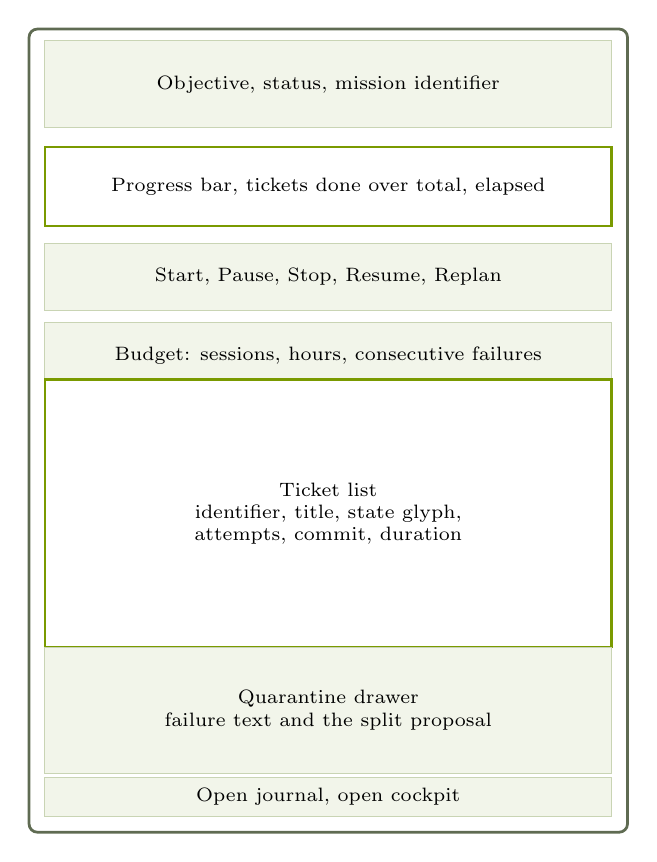
\begin{tikzpicture}[
  reg/.style={draw=xyraline,fill=xyrapanel,font=\scriptsize,align=center},
  hi/.style={draw=xyralime,line width=0.9pt,fill=white,font=\scriptsize,align=center}
]
\draw[draw=xyragrey,line width=1pt,rounded corners=3pt] (0,0) rectangle (7.6,10.2);
\node[reg,minimum width=7.2cm,minimum height=1.1cm] at (3.8,9.5) {Objective, status, mission identifier};
\node[hi,minimum width=7.2cm,minimum height=1.0cm] at (3.8,8.2) {Progress bar, tickets done over total, elapsed};
\node[reg,minimum width=7.2cm,minimum height=0.85cm] at (3.8,7.05) {Start, Pause, Stop, Resume, Replan};
\node[reg,minimum width=7.2cm,minimum height=0.85cm] at (3.8,6.05) {Budget: sessions, hours, consecutive failures};
\node[hi,minimum width=7.2cm,minimum height=3.4cm] at (3.8,4.05) {Ticket list\\identifier, title, state glyph,\\attempts, commit, duration};
\node[reg,minimum width=7.2cm,minimum height=1.6cm] at (3.8,1.55) {Quarantine drawer\\failure text and the split proposal};
\node[reg,minimum width=7.2cm,minimum height=0.5cm] at (3.8,0.45) {Open journal, open cockpit};
\end{tikzpicture}
\caption{Mission Control layout.}
\end{figure}

\begin{longtable}{@{}p{0.28\textwidth} p{0.18\textwidth} p{0.46\textwidth}@{}}
\toprule
\textbf{Control} & \textbf{Label} & \textbf{Behaviour} \\
\midrule
\endhead
ctl.mission.objective & Objective field & Multi line, editable before start, read only during a run \\
ctl.mission.plan & Plan & Produces the ticket graph without executing, so it can be reviewed \\
ctl.mission.start & Start & Plans if needed, then runs to completion \\
ctl.mission.pause & Pause & Halts after the ticket in flight, state preserved \\
ctl.mission.resume & Resume & Continues from durable state, also available after a crash \\
ctl.mission.stop & Stop & Halts and marks the mission stopped \\
ctl.mission.background & Run in background & Detaches the supervisor so it survives closing the window \\
ctl.mission.budget & Budget & Popover with sessions, hours, attempts per ticket, consecutive failures \\
ctl.mission.ticket & Ticket row & Click opens the ticket detail: brief, diff, verification output, transcript \\
ctl.mission.retry & Retry ticket & Requeues a quarantined ticket, optionally with a different vendor \\
ctl.mission.split & Split ticket & Sends the ticket to the replanner and inserts the children \\
ctl.mission.skip & Skip ticket & Marks it abandoned and unblocks its dependants where possible \\
ctl.mission.edit & Edit ticket & Modifies title, scope and files before it runs \\
ctl.mission.reorder & Drag handle & Reorders within the constraints of the dependency graph \\
ctl.mission.addticket & Add ticket & Inserts a manual ticket into the graph \\
ctl.mission.journal & Open journal & Opens the decision journal filtered to this mission \\
ctl.mission.cockpit & Open cockpit & Opens the end of mission summary and the approval gate \\
\bottomrule
\caption{Mission Control controls.}
\end{longtable}

\subsection{Ticket states}

\begin{table}[h]
\centering
\small
\begin{tabularx}{\textwidth}{l l X}
\toprule
\textbf{State} & \textbf{Glyph} & \textbf{Meaning} \\
\midrule
pending & Hollow circle & Waiting for its dependencies \\
ready & Outlined circle & Dependencies satisfied, queued \\
running & Filled ring, animated & A session is executing it now \\
verifying & Half filled ring & Session finished, tests executing in a snapshot \\
done & Check & Verified and committed, commit hash shown \\
retry & Rotating arrow & Failed, queued again with a different vendor \\
split & Branch glyph & Replaced by children \\
quarantined & Warning triangle & Exhausted its policy, needs a human \\
skipped & Dash & Abandoned deliberately \\
\bottomrule
\end{tabularx}
\caption{Ticket state vocabulary. Every state has a glyph, a colour and a word.}
\end{table}

\section{Agent Theatre}

\begin{figure}[h]
\centering
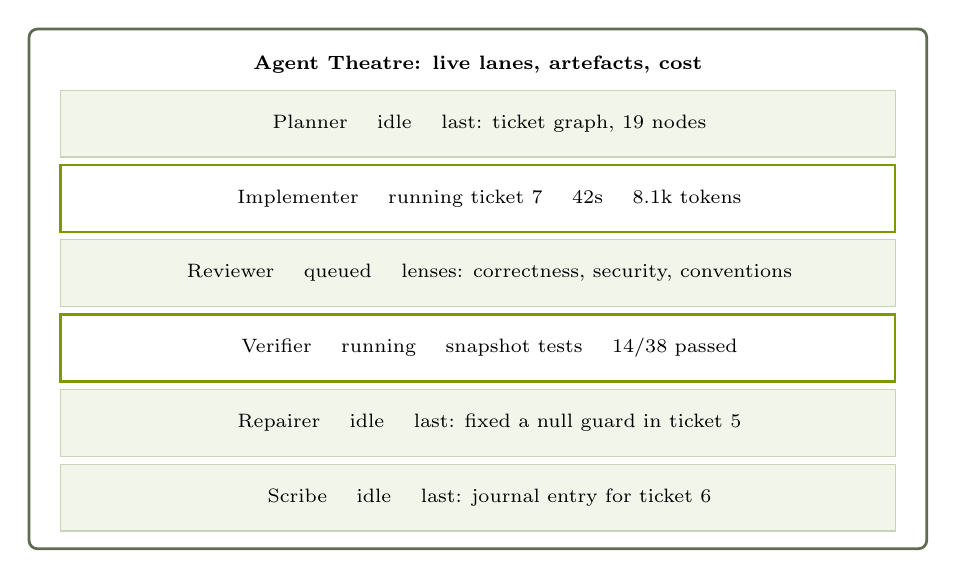
\begin{tikzpicture}[
  lane/.style={draw=xyraline,fill=xyrapanel,minimum width=10.6cm,minimum height=0.85cm,font=\scriptsize,align=left},
  hi/.style={draw=xyralime,line width=0.9pt,fill=white,minimum width=10.6cm,minimum height=0.85cm,font=\scriptsize,align=left}
]
\draw[draw=xyragrey,line width=1pt,rounded corners=3pt] (0,0) rectangle (11.4,6.6);
\node[font=\scriptsize\bfseries] at (5.7,6.15) {Agent Theatre: live lanes, artefacts, cost};
\node[lane] at (5.7,5.4) {\hspace{2mm} Planner \quad idle \quad last: ticket graph, 19 nodes};
\node[hi] at (5.7,4.45) {\hspace{2mm} Implementer \quad running ticket 7 \quad 42s \quad 8.1k tokens};
\node[lane] at (5.7,3.5) {\hspace{2mm} Reviewer \quad queued \quad lenses: correctness, security, conventions};
\node[hi] at (5.7,2.55) {\hspace{2mm} Verifier \quad running \quad snapshot tests \quad 14/38 passed};
\node[lane] at (5.7,1.6) {\hspace{2mm} Repairer \quad idle \quad last: fixed a null guard in ticket 5};
\node[lane] at (5.7,0.65) {\hspace{2mm} Scribe \quad idle \quad last: journal entry for ticket 6};
\end{tikzpicture}
\caption{Agent Theatre. One lane per role from Table~\ref{tab:roles}, each showing its current
act and its last artefact. Architect and Replanner lanes appear only while those roles are
active, so an idle mission shows six lanes rather than eight.}
\end{figure}

\begin{longtable}{@{}p{0.28\textwidth} p{0.64\textwidth}@{}}
\toprule
\textbf{Control} & \textbf{Behaviour} \\
\midrule
\endhead
ctl.theatre.lane & Expands to the lane's transcript, tool calls and produced artefacts \\
ctl.theatre.artifact & Opens the artefact: a diff, a verdict, a screenshot, a report \\
ctl.theatre.kill & Terminates the session in that lane and marks its ticket failed \\
ctl.theatre.vendor & Switches the vendor for that role for subsequent sessions \\
ctl.theatre.follow & Follows the active lane automatically as work moves between roles \\
ctl.theatre.cost & Toggles the cost column between tokens, requests and elapsed \\
ctl.theatre.graph & Switches from lanes to a node graph showing which role handed work to which \\
ctl.theatre.filter & Filters lanes by role or by ticket \\
\bottomrule
\caption{Agent Theatre controls.}
\end{longtable}

\section{Context Inspector}

\begin{longtable}{@{}p{0.28\textwidth} p{0.64\textwidth}@{}}
\toprule
\textbf{Control} & \textbf{Behaviour} \\
\midrule
\endhead
ctl.context.budget & Budget bar: used versus available, segmented by tier, with the token count \\
ctl.context.item & One row per included item: path, tier, tokens, why it was included \\
ctl.context.why & Explains the inclusion reason: structural closure, pinned, similarity fallback, skill \\
ctl.context.pin & Pins an item so the solver must always include it \\
ctl.context.exclude & Excludes an item for this workspace and writes the rule to settings \\
ctl.context.expand & Raises an item's tier, for example from signatures to full body \\
ctl.context.collapse & Lowers an item's tier to reclaim budget \\
ctl.context.heat & Heat map over the file tree, coloured by accumulated agent attention \\
ctl.context.skills & Lists the skills injected into the current session with their source \\
ctl.context.integrations & Shows which expansion integrations contributed, with a capability toggle each \\
ctl.context.compression & Shows the compression ratio and the escalation rate for the session \\
ctl.context.export & Exports the exact assembled context for reproduction and debugging \\
\bottomrule
\caption{Context Inspector controls.}
\end{longtable}

\section{Verification Deck}

\begin{longtable}{@{}p{0.28\textwidth} p{0.64\textwidth}@{}}
\toprule
\textbf{Control} & \textbf{Behaviour} \\
\midrule
\endhead
ctl.verify.run & Verify now: snapshots the change set and runs the mapped tests \\
ctl.verify.full & Full suite: runs everything rather than the mapped subset \\
ctl.verify.result & A run: command, exit code, duration, failing tests, output tail \\
ctl.verify.rerun & Reruns a single failing test in isolation \\
ctl.verify.repair & Hands the failure to the repairer inside the snapshot \\
ctl.verify.visual & Renders the configured page and returns a visual verdict \\
ctl.verify.compare & Compares the render against a design export \\
ctl.verify.qa & Runs an adversarial sweep against the running application \\
ctl.verify.flags & Security and cost flags with severity, file and line \\
ctl.verify.policy & Opens the verification policy for this repository \\
ctl.verify.history & Previous runs with their verdicts, filterable by ticket \\
\bottomrule
\caption{Verification Deck controls.}
\end{longtable}

\section{Atlas}

\begin{longtable}{@{}p{0.28\textwidth} p{0.64\textwidth}@{}}
\toprule
\textbf{Control} & \textbf{Behaviour} \\
\midrule
\endhead
ctl.atlas.mode & Switches between topology, impact, ownership and history views \\
ctl.atlas.filter & Filters nodes by path, language or module \\
ctl.atlas.focus & Focuses a node and dims everything outside its neighbourhood \\
ctl.atlas.depth & Sets transitive depth for impact, from one to unbounded \\
ctl.atlas.open & Opens the file at the definition \\
ctl.atlas.mission & Creates a mission scoped to the current selection \\
ctl.atlas.fleet & Switches the scope from this repository to the registered fleet \\
ctl.atlas.export & Exports the current view as a vector image for documentation \\
\bottomrule
\caption{Atlas controls.}
\end{longtable}

\section{Status bar}

\begin{table}[h]
\centering
\small
\begin{tabularx}{\textwidth}{l X}
\toprule
\textbf{Control} & \textbf{Behaviour} \\
\midrule
ctl.status.panels & Labelled toggles: Files, Search, Git, Mission, Agents, Context, Verify, Terminal \\
ctl.status.diag & Errors and warnings, click opens Problems \\
ctl.status.verify & Last verification verdict with a glyph, click opens the Deck \\
ctl.status.tokens & Tokens used in the current session and the budget remaining \\
ctl.status.cost & Session cost when the provider reports it, otherwise request count \\
ctl.status.ekg & Activity pulse driven by real agent state: idle, thinking, verifying, failing \\
ctl.status.position & Cursor position, selection size, indentation, encoding, language \\
\bottomrule
\end{tabularx}
\caption{Status bar controls.}
\end{table}

\section{Command palette and decisions}

The palette is the universal entry point and is required to reach every command in this
document. It supports three modes: commands, symbols with a leading hash, and files with a
leading slash. Missions are startable directly from it with a leading exclamation mark.

Decision cards replace terminal questions. When an agent reaches a genuine fork it emits a
choice, and the interface renders two or three cards side by side, each carrying the option
name, its measured cost, its structural consequence and a code sketch. Selecting a card
records the decision in the journal with its rationale and resumes the mission.

\section{First run}

\begin{enumerate}
  \item Welcome: product statement, open a project, clone from a provider.
  \item Model routing: choose the implementer, the reviewer, the planner and the embedding
  model, with a local only option offered explicitly.
  \item Sign in to the chosen providers, each with its own state indicator.
  \item Index the project, showing determinate progress and what is being built.
  \item Optional fleet registration.
  \item A guided first mission on a scoped objective, so the developer sees the whole loop
  before trusting it with real work.
\end{enumerate}

\section{Keymap}

\begin{table}[h]
\centering
\small
\begin{tabularx}{\textwidth}{l X}
\toprule
\textbf{Binding} & \textbf{Command} \\
\midrule
mod+shift+p & Command palette \\
mod+p & Files \\
mod+shift+f & Search across the project \\
mod+i & Inline agent prompt at the cursor \\
mod+m & Toggle Mission Control \\
mod+shift+m & Start or resume the mission \\
mod+alt+m & Stop the mission \\
mod+g & Toggle Agent Theatre \\
mod+k then c & Toggle Context Inspector \\
mod+shift+v & Verify now \\
mod+alt+v & Full verification \\
mod+shift+a & Toggle Atlas \\
mod+alt+i & Impact for the symbol under the cursor \\
mod+j & Toggle terminal \\
mod+enter & Accept the agent range under the cursor \\
mod+backspace & Revert the agent range under the cursor \\
\bottomrule
\end{tabularx}
\caption{Default bindings. Every one is rebindable and every command is reachable without one.}
\end{table}

\section{States that must be designed, not improvised}

\begin{longtable}{@{}p{0.26\textwidth} p{0.66\textwidth}@{}}
\toprule
\textbf{State} & \textbf{Requirement} \\
\midrule
\endhead
Empty project & Explains what to do next with a primary action, never a blank pane \\
Indexing & Determinate progress, the product remains usable, agents wait rather than guess \\
No model configured & Blocks agent surfaces with a direct route to routing settings \\
Provider unauthenticated & Inline sign in with the exact command, never a silent failure \\
Mission running & Every surface shows it, and closing the window does not kill it \\
Verification failing & Failure is the loudest thing on screen, with the exact command to reproduce \\
Quarantined ticket & Failure text and the proposed split, with one click to accept the split \\
Offline & Local capabilities keep working and remote ones are visibly disabled \\
Large repository & Progressive indexing, structural queries available before embeddings finish \\
Conflicting edits & The developer's edit always wins, the agent range is marked stale and reverifies \\
\bottomrule
\caption{Designed states.}
\end{longtable}

\chapter{User Stories}
\label{ch:stories}

Every story below is written from a persona, states the value, and carries acceptance
criteria that an implementation can be tested against. Each story names the surfaces from
Chapter~\ref{ch:interface} it exercises, which is what keeps the interface specification
honest: a surface with no story behind it should not exist.

\section{Personas}

\begin{table}[h]
\centering
\small
\begin{tabularx}{\textwidth}{l X}
\toprule
\textbf{Persona} & \textbf{Context and pressure} \\
\midrule
Solo founder & Owns the entire stack, works in bursts, cannot afford a wrong autonomous change reaching production \\
Staff engineer & Large existing codebase, cares about blast radius and review quality more than raw speed \\
Team lead & Wants the team's standards enforced mechanically rather than in review comments \\
Contractor & Enters unfamiliar repositories constantly, needs orientation before change \\
Regulated team & Must show what changed, who decided it, what verified it, and what left the machine \\
\bottomrule
\end{tabularx}
\caption{Personas driving the specification.}
\end{table}

\section{Orientation and understanding}

\begin{story}{S-01 \quad Understand an unfamiliar repository}
As a contractor, I open a repository I have never seen and want a structural orientation
rather than a folder listing.
\end{story}
\begin{itemize}
  \item Atlas opens on the topology view with modules grouped and entry points marked.
  \item Structural queries are answerable before embedding indexing completes.
  \item Selecting any node shows what it imports, what imports it, and the symbols it defines.
  \item Surfaces: Atlas, Workbench.
\end{itemize}

\begin{story}{S-02 \quad Know the blast radius before changing a shared contract}
As a staff engineer, before I rename a function used across the codebase I want the exact set
of files that will break, not a guess.
\end{story}
\begin{itemize}
  \item Impact for the symbol under the cursor returns the definition, importers by
  transitive distance, and textual references.
  \item The result is computed from parsed imports, and the interface states that it is
  deterministic.
  \item If a similarity fallback contributed any row, that row is labelled as a guess.
  \item Surfaces: Workbench inline, Atlas.
\end{itemize}

\begin{story}{S-03 \quad See why a line exists before deleting it}
As a staff engineer, when an agent proposes removing code I want the history that explains it.
\end{story}
\begin{itemize}
  \item Blame is available inline without leaving the buffer.
  \item The agent's context for that region included the commit message that introduced it.
  \item The Context Inspector shows history as a contributing integration.
  \item Surfaces: Workbench gutter, Context Inspector.
\end{itemize}

\section{Assisted change}

\begin{story}{S-04 \quad Make a small change and trust it}
As a solo founder, I ask for a small change and want to see only code that already runs.
\end{story}
\begin{itemize}
  \item The change is executed against the project's own test command in an isolated snapshot
  before it is displayed.
  \item The displayed diff carries the verification verdict, the command and the exit code.
  \item If verification failed, the failure is shown instead of the diff, with the exact
  command to reproduce it.
  \item My working tree was never modified during verification.
  \item Surfaces: Workbench, Verification Deck.
\end{itemize}

\begin{story}{S-05 \quad Correct an agent range without losing my own edits}
As any developer, I edit a file while an agent is working in it.
\end{story}
\begin{itemize}
  \item My edit always wins; the agent range is marked stale rather than overwritten.
  \item The stale range is reverified before it can be accepted.
  \item Accept and revert are available per range, not only per file.
  \item Surfaces: Workbench gutter and inline controls.
\end{itemize}

\begin{story}{S-06 \quad Get a rival opinion on a risky diff}
As a team lead, before merging a change to a payment path I want an adversarial review from a
different vendor.
\end{story}
\begin{itemize}
  \item Review runs three lenses in parallel and returns a structured verdict with severities.
  \item Repository policy can require extra lenses and a lower blocking threshold for
  configured paths.
  \item The verdict is stored in the journal and can be exported for an audit.
  \item Surfaces: Verification Deck, Agent Theatre.
\end{itemize}

\section{Autonomous delivery}

\begin{story}{S-07 \quad Ship a whole feature while I am away}
As a solo founder, I state an objective, leave, and return to finished work.
\end{story}
\begin{itemize}
  \item The objective is decomposed into a dependency ordered ticket graph I can review before
  execution.
  \item Each ticket executes in a fresh session, is verified, and is committed separately.
  \item No prompt, question or confirmation is required for anything the supervisor can decide.
  \item Progress is visible at a glance from the title bar without opening a panel.
  \item Surfaces: Mission Control, Agent Theatre, Verification Deck.
\end{itemize}

\begin{story}{S-08 \quad Survive a failure without losing the run}
As a solo founder, one ticket fails repeatedly and I do not want the mission to stop.
\end{story}
\begin{itemize}
  \item The supervisor retries, then swaps vendor, then splits the ticket into smaller
  children, then quarantines it.
  \item Work that does not depend on the quarantined ticket continues.
  \item The quarantine entry shows the failure text and the proposed split, and accepting the
  split is one action.
  \item Surfaces: Mission Control.
\end{itemize}

\begin{story}{S-09 \quad Close the laptop mid mission}
As any developer, I close the machine during a long run.
\end{story}
\begin{itemize}
  \item Mission state is durable and resuming continues from the last completed ticket.
  \item At most the ticket in flight is lost, and its partial work is discarded rather than
  committed.
  \item Resuming requires one action and no re planning.
  \item Surfaces: Mission Control.
\end{itemize}

\begin{story}{S-10 \quad Stop a mission immediately}
As any developer, I decide the mission is going the wrong way.
\end{story}
\begin{itemize}
  \item Stop halts after the ticket in flight, leaving the repository in a committed state.
  \item Everything already committed remains, and the journal explains what each commit did.
  \item Restarting with a corrected objective does not require undoing the good work.
  \item Surfaces: Mission Control, title bar.
\end{itemize}

\begin{story}{S-11 \quad Cap the cost of autonomy}
As a team lead, I need a hard ceiling on an unattended run.
\end{story}
\begin{itemize}
  \item Sessions, wall clock hours, attempts per ticket and consecutive failures are all
  capped and editable before and during a run.
  \item Reaching a cap halts the mission with a stated reason rather than continuing.
  \item Token and cost usage are visible while the run proceeds.
  \item Surfaces: Mission Control, status bar.
\end{itemize}

\section{Correctness of appearance}

\begin{story}{S-12 \quad Verify a page actually looks right}
As a solo founder, after a styling change I want the machine to look at the result.
\end{story}
\begin{itemize}
  \item The page is rendered headless, screenshotted, and judged against a stated intent.
  \item The verdict is structured with issues ranked by severity, so it can drive a fix loop.
  \item High severity issues trigger an automatic repair attempt before the change is
  presented.
  \item Surfaces: Verification Deck.
\end{itemize}

\begin{story}{S-13 \quad Match an intended design}
As a team lead, the implementation must match the design export.
\end{story}
\begin{itemize}
  \item A design image can be attached to a ticket or supplied ad hoc.
  \item Comparison returns concrete differences: layout shifts, missing elements, wrong
  colours, spacing.
  \item Differences become tickets rather than a wall of prose.
  \item Surfaces: Verification Deck, Mission Control.
\end{itemize}

\section{Scale and cross repository work}

\begin{story}{S-14 \quad Change a contract across repositories}
As a staff engineer, an endpoint changes in the backend and every consumer must follow.
\end{story}
\begin{itemize}
  \item Fleet impact separates the defining repository from consuming ones.
  \item Execution proceeds in dependency order, verifying each repository independently.
  \item Related changes are prepared together and linked.
  \item Surfaces: Atlas in fleet scope, Mission Control.
\end{itemize}

\begin{story}{S-15 \quad Register the fleet without editing configuration}
As any developer, I want to pick my repositories from my provider rather than write a manifest.
\end{story}
\begin{itemize}
  \item Repositories are listed from the authenticated provider.
  \item Selected repositories that are missing locally are cloned.
  \item Roles are proposed automatically and remain editable.
  \item Surfaces: Atlas, first run.
\end{itemize}

\section{Control over the machine}

\begin{story}{S-16 \quad See exactly what the agent is reading}
As a staff engineer, when output is wrong I want to know what the model was looking at.
\end{story}
\begin{itemize}
  \item Every included item is listed with its tier, its token cost and its inclusion reason.
  \item Items included by similarity are labelled distinctly from structural inclusions.
  \item Any item can be pinned or excluded, and exclusions persist for the workspace.
  \item The exact assembled context can be exported and replayed.
  \item Surfaces: Context Inspector.
\end{itemize}

\begin{story}{S-17 \quad Keep attention off the wrong files}
As a staff engineer, generated files dominate attention and produce noise.
\end{story}
\begin{itemize}
  \item The attention heat map shows which files accumulate agent reads.
  \item Excluding a file or a glob is one action from the heat map.
  \item The exclusion applies to future context assembly immediately, without reindexing.
  \item Surfaces: Context Inspector.
\end{itemize}

\begin{story}{S-18 \quad Decide an architectural fork deliberately}
As a team lead, when the agent reaches a real decision I want to choose with costs in front of me.
\end{story}
\begin{itemize}
  \item The choice is presented as cards, each with measured cost and structural consequence.
  \item Unblocked tickets continue while the choice is pending.
  \item The decision and its rationale are recorded in the journal.
  \item Surfaces: decision cards, Mission Control.
\end{itemize}

\begin{story}{S-19 \quad Return to a past decision and take the other branch}
As a staff engineer, a decision three commits back turned out wrong.
\end{story}
\begin{itemize}
  \item The journal shows decisions on a timeline anchored to commits.
  \item Branching from a decision point is one action and does not disturb the current tree.
  \item The alternative can be run as a new mission scoped to that branch.
  \item Surfaces: Atlas history view, Mission Control.
\end{itemize}

\section{Team standards and compliance}

\begin{story}{S-20 \quad Enforce house standards without review comments}
As a team lead, every agent session in this repository must follow our conventions.
\end{story}
\begin{itemize}
  \item Workspace skills override user skills of the same name.
  \item The Context Inspector shows which skills were injected and from where.
  \item A violation is caught by the reviewer lens rather than by a human in review.
  \item Surfaces: Context Inspector, Verification Deck.
\end{itemize}

\begin{story}{S-21 \quad Prove what happened for an audit}
As a regulated team, I must show what changed, who decided it and what verified it.
\end{story}
\begin{itemize}
  \item Every ticket has a commit, a verification record and a journal entry.
  \item Review verdicts are exportable in a machine readable interchange format.
  \item Secrets are redacted before any content leaves the machine, and the redaction is
  recorded.
  \item Surfaces: Verification Deck, journal export.
\end{itemize}

\begin{story}{S-22 \quad Know what leaves the machine}
As a regulated team, I must control every outbound integration.
\end{story}
\begin{itemize}
  \item Each context expansion integration is a capability with an explicit toggle.
  \item The Context Inspector shows which integrations contributed to a session.
  \item A fully local configuration is selectable in first run and remains functional.
  \item Surfaces: Context Inspector, settings.
\end{itemize}

\section{Reliability of the tool itself}

\begin{story}{S-23 \quad Never lose the editor to an agent}
As any developer, an agent process hangs.
\end{story}
\begin{itemize}
  \item The interface stays responsive because agents run out of process.
  \item An inactivity watchdog terminates the session and marks the ticket failed.
  \item Editing, search and navigation continue unaffected.
  \item Surfaces: all.
\end{itemize}

\begin{story}{S-24 \quad Never hang on an interactive command}
As any developer, an agent runs a command that asks a question.
\end{story}
\begin{itemize}
  \item Interactive commands are refused by policy, with the non interactive form stated.
  \item Long running processes are started detached and their logs are read instead.
  \item A command producing no output for a bounded period is terminated.
  \item Surfaces: terminal, Agent Theatre.
\end{itemize}

\begin{story}{S-25 \quad Keep working while a mission runs}
As any developer, I want to edit while the supervisor works.
\end{story}
\begin{itemize}
  \item Verification runs in snapshots, so it never locks the working tree.
  \item Indexing is bounded so the machine stays usable.
  \item Conflicts between my edits and agent ranges are surfaced, never silently merged.
  \item Surfaces: Workbench, Mission Control.
\end{itemize}

\chapter{Work Breakdown and Issue Register}
\label{ch:breakdown}

\section{Categories}

Work is partitioned into twelve categories. Each category maps to a crate set from
Chapter~\ref{ch:architecture} and owns a slice of the interface from
Chapter~\ref{ch:interface}. The partition is chosen so that two categories can be worked in
parallel without editing the same files.

\begin{longtable}{@{}p{0.06\textwidth} p{0.22\textwidth} p{0.30\textwidth} p{0.34\textwidth}@{}}
\toprule
\textbf{Key} & \textbf{Category} & \textbf{Crates} & \textbf{Owns} \\
\midrule
\endhead
PLA & Platform & xyra-ui, xyra-proto, xyra-memory, xyrad, xyra & Window, element model, service wiring, storage, packaging \\
TXT & Text core & xyra-text & Rope, transactions, undo, selections \\
SYN & Syntax & xyra-syntax & Parsing, highlighting, structural motion \\
LNG & Language & xyra-lang & Language servers, diagnostics, completion, refactors \\
PRJ & Project & xyra-project, xyra-vcs & Worktree, watching, git \\
TRM & Terminal & xyra-term & Terminal grid, process supervision \\
CTX & Context engine & xyra-context & Graph, retrieval, compression, budget solver \\
AGT & Agent layer & xyra-agent, xyra-skills & Sessions, protocols, tools, skills \\
MIS & Mission & xyra-mission & Ticket graph, supervisor, budgets, journal \\
VER & Verification & xyra-verify & Sandbox, visual checks, sweeps, flags \\
FLT & Fleet & xyra-fleet & Multi repository registry and operations \\
EXT & Extensions & xyra-ext & Extension host, capabilities, marketplace client \\
\bottomrule
\caption{Work categories and their ownership boundaries.}
\end{longtable}

\section{Dependency between categories}

\begin{figure}[h]
\centering
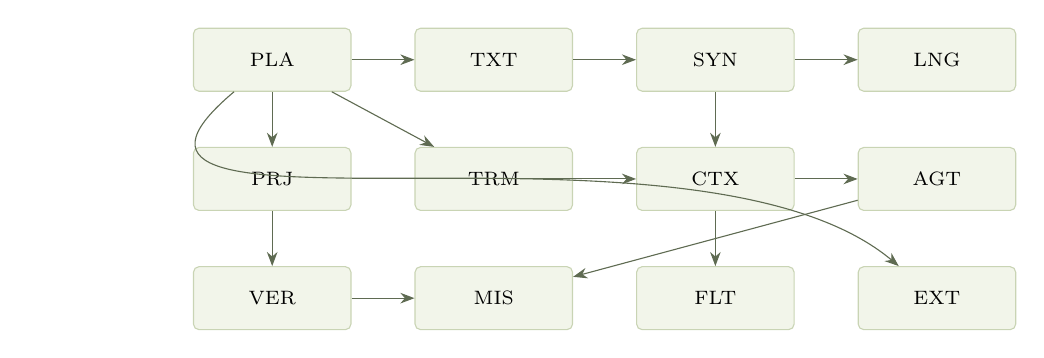
\begin{tikzpicture}[
  cat/.style={draw=xyraline,fill=xyrapanel,rounded corners=2pt,minimum height=8mm,minimum width=20mm,font=\scriptsize},
  arr/.style={-{Stealth[length=1.8mm]},xyragrey}
]
\node[cat] (pla) at (0,0) {PLA};
\node[cat,right=8mm of pla] (txt) {TXT};
\node[cat,right=8mm of txt] (syn) {SYN};
\node[cat,right=8mm of syn] (lng) {LNG};
\node[cat,below=7mm of pla] (prj) {PRJ};
\node[cat,right=8mm of prj] (trm) {TRM};
\node[cat,right=8mm of trm] (ctx) {CTX};
\node[cat,right=8mm of ctx] (agt) {AGT};
\node[cat,below=7mm of prj] (ver) {VER};
\node[cat,right=8mm of ver] (mis) {MIS};
\node[cat,right=8mm of mis] (flt) {FLT};
\node[cat,right=8mm of flt] (ext) {EXT};

\draw[arr] (pla) -- (txt);
\draw[arr] (txt) -- (syn);
\draw[arr] (syn) -- (lng);
\draw[arr] (pla) -- (prj);
\draw[arr] (prj) -- (ctx);
\draw[arr] (syn) -- (ctx);
\draw[arr] (ctx) -- (agt);
\draw[arr] (prj) -- (ver);
\draw[arr] (agt) -- (mis);
\draw[arr] (ver) -- (mis);
\draw[arr] (ctx) -- (flt);
\draw[arr] (pla) -- (trm);
\draw[arr] (pla) to[out=-140,in=140] (ext);
\end{tikzpicture}
\caption{Category dependencies. Anything not connected can proceed in parallel.}
\end{figure}

\section{Issue register}

Identifiers are stable and are referenced by the generation prompts in
Chapter~\ref{ch:prompts}. The Depends column lists issues that must land first.

\begin{longtable}{@{}p{0.09\textwidth} p{0.55\textwidth} p{0.28\textwidth}@{}}
\toprule
\textbf{ID} & \textbf{Issue} & \textbf{Depends} \\
\midrule
\endfirsthead
\toprule
\textbf{ID} & \textbf{Issue} & \textbf{Depends} \\
\midrule
\endhead

\multicolumn{3}{@{}l}{\textbf{PLA \quad Platform}}\\
PLA-001 & Repository skeleton, workspace manifest, lint and format configuration, license allow list check, continuous integration definition & \\
PLA-002 & Vendor the UI framework at a pinned revision with its license intact & PLA-001 \\
PLA-003 & Extend the license check to vendored third party trees and generate the aggregated notice file & PLA-002 \\
PLA-004 & xyra-ui: element primitives, flex containers, text, icon, scroll area & PLA-002 \\
PLA-005 & xyra-ui: theme tokens from Chapter six, light and dark & PLA-004 \\
PLA-006 & xyra-ui: button, input, select, checkbox, toggle, slider with all states & PLA-005 \\
PLA-007 & xyra-ui: list with virtualisation and keyboard navigation & PLA-004 \\
PLA-008 & xyra-ui: table with sortable columns and sticky header & PLA-007 \\
PLA-009 & xyra-ui: popover, dropdown, context menu, tooltip & PLA-006 \\
PLA-010 & xyra-ui: modal dialog, confirmation, and focus trapping & PLA-009 \\
PLA-011 & xyra-ui: toast and notification centre & PLA-009 \\
PLA-012 & xyra-ui: progress bar, determinate and indeterminate, and the activity pulse & PLA-006 \\
PLA-013 & Window shell: title bar, activity bar, docks, resizable splits & PLA-004 \\
PLA-014 & Dock persistence: sizes, visibility and active panel per workspace & PLA-013 \\
PLA-015 & xyra-proto: message types, versioning, backward compatible decoding & PLA-001 \\
PLA-016 & xyrad service: supervision tree, graceful shutdown, restart policy & PLA-015 \\
PLA-017 & Interface to service transport over a local socket with reconnect & PLA-016 \\
PLA-018 & Projection dispatch with version stamps and stale frame rejection & PLA-017 \\
PLA-019 & Intent routing from surfaces to the core reducer & PLA-018 \\
PLA-020 & Settings: layered defaults, user and workspace, live reload & PLA-016 \\
PLA-021 & Command registry and the command palette with three modes & PLA-009 \\
PLA-022 & Keymap engine, rebinding, conflict detection, chord support & PLA-021 \\
PLA-023 & Storage layer: embedded stores, migrations, integrity checks & PLA-016 \\
PLA-024 & Crash reporting that is local by default and opt in for upload & PLA-016 \\
PLA-025 & Packaging for macOS, Linux and Windows with signed artefacts & PLA-013 \\
PLA-026 & Update channel with staged rollout and rollback & PLA-025 \\
PLA-027 & Accessibility layer: names, roles, focus order, screen reader output & PLA-006 \\
PLA-028 & Internationalisation scaffolding with externalised strings & PLA-006 \\
PLA-029 & Headless mode for the core service to run without a window & PLA-016 \\
PLA-030 & Interface test harness driving projections and asserting intents & PLA-019 \\

\multicolumn{3}{@{}l}{\textbf{TXT \quad Text core}}\\
TXT-001 & Rope buffer with line and character indexing & PLA-001 \\
TXT-002 & Edit transactions with grouping and coalescing & TXT-001 \\
TXT-003 & Undo and redo history with selection restoration & TXT-002 \\
TXT-004 & Multi cursor and multi selection algebra & TXT-002 \\
TXT-005 & Word, line, paragraph and bracket motions & TXT-004 \\
TXT-006 & Encoding detection and line ending preservation & TXT-001 \\
TXT-007 & Large file strategy with chunked loading and disabled features & TXT-001 \\
TXT-008 & Search within a buffer, literal and regular expression & TXT-001 \\
TXT-009 & Replace with preview and per match acceptance & TXT-008 \\
TXT-010 & Soft wrap, virtual whitespace and indentation guides & TXT-001 \\
TXT-011 & External change detection and non destructive reload & TXT-001 \\
TXT-012 & Buffer transaction fuzz harness & TXT-003 \\

\multicolumn{3}{@{}l}{\textbf{SYN \quad Syntax}}\\
SYN-001 & Parser host with incremental reparse on edit & TXT-002 \\
SYN-002 & Grammar loading and per language configuration & SYN-001 \\
SYN-003 & Highlight queries mapped to theme tokens & SYN-002, PLA-005 \\
SYN-004 & Bracket matching and auto closing pairs & SYN-001 \\
SYN-005 & Structural selection expand and shrink & SYN-001 \\
SYN-006 & Code folding by syntax node & SYN-001 \\
SYN-007 & Indentation rules derived from the grammar & SYN-002 \\
SYN-008 & Symbol extraction feeding the context engine & SYN-001 \\
SYN-009 & Injection support for embedded languages & SYN-002 \\
SYN-010 & Breadcrumb path from the parse tree & SYN-008 \\

\multicolumn{3}{@{}l}{\textbf{LNG \quad Language}}\\
LNG-001 & Language server process supervision with restart backoff & PLA-016 \\
LNG-002 & Capability negotiation and per server feature gating & LNG-001 \\
LNG-003 & Diagnostics ingestion, deduplication and gutter rendering & LNG-002 \\
LNG-004 & Completion with resolve, snippets and sorting & LNG-002 \\
LNG-005 & Hover with type information rendered as structured content & LNG-002 \\
LNG-006 & Go to definition, declaration, type definition and implementation & LNG-002 \\
LNG-007 & Find references with a grouped result surface & LNG-006 \\
LNG-008 & Rename symbol with a preview of every edit & LNG-007 \\
LNG-009 & Code actions and quick fixes & LNG-003 \\
LNG-010 & Formatting on save and on demand & LNG-002 \\
LNG-011 & Signature help & LNG-004 \\
LNG-012 & Call hierarchy exposed to the context engine & LNG-006 \\
LNG-013 & Workspace symbol search & LNG-002 \\
LNG-014 & Inlay hints with a density control & LNG-002 \\
LNG-015 & Language server output surface for debugging & LNG-001 \\

\multicolumn{3}{@{}l}{\textbf{PRJ \quad Project and version control}}\\
PRJ-001 & Worktree model with ignore aware traversal & PLA-016 \\
PRJ-002 & Filesystem watching with debouncing and rename detection & PRJ-001 \\
PRJ-003 & Explorer tree with keyboard navigation and multi select & PRJ-001, PLA-007 \\
PRJ-004 & File operations: create, rename, move, delete with undo where possible & PRJ-003 \\
PRJ-005 & Project wide search with structural filters & PRJ-001 \\
PRJ-006 & Search and replace across files with per match acceptance & PRJ-005 \\
PRJ-007 & Git status, staging and unstaging by hunk & PRJ-001 \\
PRJ-008 & Commit surface with message assistance and amend & PRJ-007 \\
PRJ-009 & Branch list, switch, create and delete & PRJ-007 \\
PRJ-010 & Diff view, split and unified, with word level highlighting & PRJ-007 \\
PRJ-011 & Blame with commit detail on hover & PRJ-007 \\
PRJ-012 & Conflict resolution surface & PRJ-010 \\
PRJ-013 & Stash operations & PRJ-007 \\
PRJ-014 & Remote operations: fetch, pull, push with authentication handling & PRJ-009 \\
PRJ-015 & History view feeding the Atlas history mode & PRJ-011 \\

\multicolumn{3}{@{}l}{\textbf{TRM \quad Terminal}}\\
TRM-001 & Terminal grid and escape sequence handling & PLA-004 \\
TRM-002 & Process supervision with environment construction & PLA-016 \\
TRM-003 & Multiple terminals with tabs and splits & TRM-001 \\
TRM-004 & Scrollback, search and copy semantics & TRM-001 \\
TRM-005 & Task runner definitions and execution & TRM-002 \\
TRM-006 & Output capture available to agents as context & TRM-002, CTX-020 \\
TRM-007 & Non interactive policy enforcement on agent invoked commands & TRM-002 \\
TRM-008 & Detached process management for servers with log tailing & TRM-002 \\

\multicolumn{3}{@{}l}{\textbf{CTX \quad Context engine}}\\
CTX-001 & Import parsing for TypeScript and JavaScript & SYN-008 \\
CTX-002 & Import parsing for Python & SYN-008 \\
CTX-003 & Import parsing for Rust & SYN-008 \\
CTX-004 & Import parsing for Go and Java & SYN-008 \\
CTX-005 & Import resolution to concrete paths with alias support & CTX-001 \\
CTX-006 & Symbol table with kind, visibility and location & SYN-008 \\
CTX-007 & Call edge extraction per symbol & SYN-008 \\
CTX-008 & Graph storage with incremental update on file change & CTX-005, PRJ-002 \\
CTX-009 & Impact closure query with transitive distance & CTX-008 \\
CTX-010 & Neighbourhood query for a single file & CTX-008 \\
CTX-011 & Test to source mapping from imports & CTX-008 \\
CTX-012 & Test to source mapping refined by execution traces & CTX-011, VER-004 \\
CTX-013 & SCP record generation at levels zero, one and two & SYN-008 \\
CTX-014 & SCP body handles with content addressed retrieval & CTX-013 \\
CTX-015 & Token counting with the target model tokeniser & PLA-001 \\
CTX-016 & Budget solver with value, cost, redundancy and dependency & CTX-015, CTX-013 \\
CTX-017 & Inclusion floors that cannot be evicted by the solver & CTX-016 \\
CTX-018 & Delta encoding dictionary per mission & CTX-014 \\
CTX-019 & Stable emission order for provider prefix cache alignment & CTX-016 \\
CTX-020 & Context assembly pipeline end to end & CTX-019, CTX-018 \\
CTX-021 & Chunking strategy aligned to syntax nodes & SYN-008 \\
CTX-022 & Local embedding generation with incremental content hashing & CTX-021 \\
CTX-023 & Vector index, quantised and memory mapped & CTX-022 \\
CTX-024 & Similarity search labelled as a fallback in results & CTX-023 \\
CTX-025 & Local cross encoder reranking of the candidate set & CTX-024 \\
CTX-026 & Speculative prefetch driven by graph prediction & CTX-009 \\
CTX-027 & Attention accounting per file for the heat map & CTX-020 \\
CTX-028 & Context export and replay for debugging & CTX-020 \\
CTX-029 & Compression and escalation metrics with a reporting surface & CTX-020 \\
CTX-030 & Integration: version history as context & PRJ-011 \\
CTX-031 & Integration: language server hover and hierarchy as context & LNG-012 \\
CTX-032 & Integration: documentation fetch by library and version & CTX-020 \\
CTX-033 & Integration: issue tracker linkage & CTX-020 \\
CTX-034 & Integration: runtime traces and logs & TRM-006 \\
CTX-035 & Integration: database schema and pending migrations & CTX-020 \\
CTX-036 & Integration: design assets and tokens & CTX-020 \\
CTX-037 & Integration: dependency registry metadata and advisories & CTX-020 \\
CTX-038 & Capability toggles and provenance display for every integration & CTX-020 \\
CTX-039 & Secret redaction before any context leaves the machine & CTX-020 \\
CTX-040 & Context evaluation harness measuring first attempt success & CTX-029 \\

\multicolumn{3}{@{}l}{\textbf{AGT \quad Agent layer}}\\
AGT-001 & Agent process supervision with environment construction & PLA-016 \\
AGT-002 & Agent client protocol transport and session lifecycle & AGT-001 \\
AGT-003 & Model context protocol client for external tool servers & AGT-001 \\
AGT-004 & Tool surface exposure with capability gating & AGT-002 \\
AGT-005 & Tool: read file at a requested tier & CTX-013 \\
AGT-006 & Tool: structural search with labelled fallback & CTX-024 \\
AGT-007 & Tool: impact and graph queries & CTX-009 \\
AGT-008 & Tool: edit as a reversible transaction & TXT-002 \\
AGT-009 & Tool: run tests inside a snapshot & VER-002 \\
AGT-010 & Tool: verify the current change set & VER-003 \\
AGT-011 & Tool: render check and design comparison & VER-006 \\
AGT-012 & Tool: quality sweep & VER-008 \\
AGT-013 & Tool: fleet search and impact & FLT-003 \\
AGT-014 & Tool: journal a decision & MIS-014 \\
AGT-015 & Tool: escalate a decision to the developer & MIS-016 \\
AGT-016 & Transcript capture streamed to disk & AGT-002 \\
AGT-017 & Inactivity watchdog and hard kill path & AGT-001 \\
AGT-018 & Role definitions with distinct mandates and tool grants & AGT-004 \\
AGT-019 & Vendor routing per role with a runtime switch & AGT-018 \\
AGT-020 & Skill registry with workspace, user and bundled precedence & PLA-020 \\
AGT-021 & Skill injection into sessions with provenance recorded & AGT-020 \\
AGT-022 & Bundled skills: autonomy, terminal, conventions, review, safety, shipping & AGT-021 \\
AGT-023 & Inline agent prompt at the cursor & AGT-002 \\
AGT-024 & Agent range tracking with accept and revert & TXT-002, AGT-023 \\
AGT-025 & Stale range detection when the developer edits concurrently & AGT-024 \\
AGT-026 & Council: parallel lens execution with structured verdicts & AGT-019 \\
AGT-027 & Council: policy as code per repository and per path & PLA-020 \\
AGT-028 & Council: consensus modes across multiple reviewers & AGT-026 \\
AGT-029 & Verdict cache keyed by content hash & AGT-026 \\
AGT-030 & Interchange export of verdicts for external scanning & AGT-026 \\

\multicolumn{3}{@{}l}{\textbf{MIS \quad Mission}}\\
MIS-001 & Ticket schema, graph storage and atomic state persistence & PLA-023 \\
MIS-002 & Planner invocation producing a dependency ordered graph & AGT-018 \\
MIS-003 & Plan review surface before execution & MIS-002 \\
MIS-004 & Ready ticket selection respecting dependencies & MIS-001 \\
MIS-005 & Fresh session execution per ticket with a compiled brief & AGT-002, CTX-020 \\
MIS-006 & Verification gate before a ticket counts as done & VER-003 \\
MIS-007 & Commit per verified ticket with a structured message & PRJ-008 \\
MIS-008 & Retry policy with attempt accounting & MIS-005 \\
MIS-009 & Vendor swap on retry & AGT-019 \\
MIS-010 & Replanner producing child tickets with bounded depth & MIS-002 \\
MIS-011 & Quarantine with failure capture and continuation & MIS-008 \\
MIS-012 & Working tree reset between attempts that spares supervisor state & PRJ-007 \\
MIS-013 & Budget enforcement across sessions, time, attempts and failures & MIS-001 \\
MIS-014 & Decision journal anchored to commits & MIS-007 \\
MIS-015 & Stop, pause and resume with durable state & MIS-001 \\
MIS-016 & Escalation as structured decision cards & PLA-010 \\
MIS-017 & Background supervisor surviving interface restarts & PLA-029 \\
MIS-018 & Crash resume from durable state & MIS-001 \\
MIS-019 & Event stream published for the Theatre and the status bar & PLA-018 \\
MIS-020 & Mission Control surface with every control from Chapter six & PLA-013 \\
MIS-021 & Ticket detail: brief, diff, verification output, transcript & MIS-020 \\
MIS-022 & Manual ticket editing, insertion, reordering and skipping & MIS-020 \\
MIS-023 & End of mission cockpit summary with an explicit approval gate & MIS-014 \\
MIS-024 & Mission templates for recurring objectives & MIS-002 \\

\multicolumn{3}{@{}l}{\textbf{VER \quad Verification}}\\
VER-001 & Runner detection across common project types & PRJ-001 \\
VER-002 & Isolated snapshot execution in a throwaway worktree & PRJ-007 \\
VER-003 & Verification verdict with command, exit code and output tail & VER-002 \\
VER-004 & Targeted test selection from the test mapping & CTX-011 \\
VER-005 & Warm worktree pool to remove setup cost & VER-002 \\
VER-006 & Headless render and screenshot capture & PLA-016 \\
VER-007 & Visual verdict with severity ranked issues & VER-006 \\
VER-008 & Adversarial application sweep with a crawler and input generation & VER-006 \\
VER-009 & Accessibility auditing during the sweep & VER-008 \\
VER-010 & Defect deduplication and severity ranking & VER-008 \\
VER-011 & Repair loop that fixes inside the snapshot and reverifies & MIS-008 \\
VER-012 & Security pattern flags with file and line & PRJ-001 \\
VER-013 & Cost pattern flags for expensive constructs & PRJ-001 \\
VER-014 & Verification Deck surface with every control from Chapter six & PLA-013 \\
VER-015 & Verification history filterable by ticket & MIS-021 \\
VER-016 & Flake detection across repeated runs & VER-003 \\

\multicolumn{3}{@{}l}{\textbf{FLT \quad Fleet}}\\
FLT-001 & Repository registry with roles and local paths & PLA-020 \\
FLT-002 & Provider listing and cloning of selected repositories & FLT-001 \\
FLT-003 & Cross repository search & CTX-008 \\
FLT-004 & Cross repository impact separating definition from consumption & FLT-003 \\
FLT-005 & Sequenced execution across repositories with independent verification & MIS-005 \\
FLT-006 & Linked change preparation across repositories & PRJ-014 \\
FLT-007 & Fleet scope in Atlas & FLT-004 \\

\multicolumn{3}{@{}l}{\textbf{EXT \quad Extensions}}\\
EXT-001 & Extension manifest schema and validation & PLA-020 \\
EXT-002 & Sandboxed execution host with a capability list & PLA-016 \\
EXT-003 & Host interface: commands, surfaces, settings contributions & EXT-002 \\
EXT-004 & Grammar and language contributions & SYN-002 \\
EXT-005 & Theme contributions & PLA-005 \\
EXT-006 & Tool contributions exposed to agents under capability control & AGT-004 \\
EXT-007 & Context integration contributions & CTX-038 \\
EXT-008 & Local installation, enable, disable and removal & EXT-001 \\
EXT-009 & Registry client with signature verification & EXT-008 \\
EXT-010 & Failure isolation so an extension trap never affects the editor & EXT-002 \\
\bottomrule
\caption{Issue register. Identifiers are stable and referenced by the generation prompts.}
\end{longtable}

\section{Milestone composition}

Milestones are defined by capability, not by date. A milestone is complete when every issue
in it passes its acceptance criteria and the stories it claims are demonstrable end to end.

\begin{longtable}{@{}p{0.14\textwidth} p{0.44\textwidth} p{0.36\textwidth}@{}}
\toprule
\textbf{Milestone} & \textbf{Capability delivered} & \textbf{Stories demonstrable} \\
\midrule
\endhead
M0 Shell & Window, docks, palette, settings, service transport, storage & None yet, foundation only \\
M1 Editor & Open, edit, save, syntax, search, git status and diff & S-01 partially, S-03 \\
M2 Intelligence & Language servers, navigation, diagnostics, refactors & S-01, S-02 partially \\
M3 Context & Graph, SCP, budget solver, retrieval, inspector & S-02, S-16, S-17 \\
M4 Agent & Sessions, tools, inline prompt, ranges, council & S-04, S-05, S-06, S-20 \\
M5 Verification & Sandbox, targeted tests, visual checks, sweeps, deck & S-04, S-12, S-13 \\
M6 Mission & Supervisor, policy, budgets, journal, Mission Control & S-07 to S-11, S-18, S-19 \\
M7 Fleet & Registry, cross repository impact and execution & S-14, S-15 \\
M8 Platform & Packaging, updates, accessibility, extensions & S-21, S-22, S-23 to S-25 \\
\bottomrule
\caption{Milestones defined by demonstrable capability.}
\end{longtable}

\section{Definition of done}

An issue is done when all of the following hold. This list is deliberately uniform so that it
can be applied mechanically by a reviewer or by an automated gate.

\begin{enumerate}
  \item The behaviour matches this document, and any deviation is recorded as an amendment
  to this document rather than left implicit in code.
  \item Tests exist at the appropriate level and pass, including at least one test for the
  failure path.
  \item No control is reachable that is not specified in Chapter~\ref{ch:interface}.
  \item Every long running operation has a budget and a cancellation path.
  \item No new dependency was added outside the license allow list.
  \item The interface remains responsive under the operation, verified by the harness.
  \item Accessibility names and keyboard reachability exist for every new control.
\end{enumerate}

\chapter{Quality, Security and Delivery}
\label{ch:quality}

\section{Testing strategy}

\begin{table}[h]
\centering
\small
\begin{tabularx}{\textwidth}{l X l}
\toprule
\textbf{Level} & \textbf{What it covers} & \textbf{Gate} \\
\midrule
Unit & Pure logic: rope operations, solver, graph queries, policy decisions & Every commit \\
Property & Invariants under random input: edits, undo, selections, graph consistency & Every commit \\
Golden & Compression output, SCP records, context assembly for fixture repositories & Every commit \\
Integration & Service and interface across the transport, with real stores & Every commit \\
Interface & Surfaces driven by projections, asserting emitted intents, no window & Every commit \\
End to end & A real mission on a fixture repository with a scripted agent & Every merge \\
Live & A real mission with a real model provider on a sample project & Before release \\
Soak & A long mission with induced failures and a killed process & Before release \\
\bottomrule
\end{tabularx}
\caption{Test levels and when each gate runs.}
\end{table}

Two rules matter more than coverage numbers. Every failure path has a test, because failure
handling is the product. And every test that touches an agent uses a scripted agent by
default, so the suite is deterministic and free; real providers appear only in the live gate.

\section{Performance budgets}

Budgets are enforced by an automated benchmark that fails the build on regression beyond the
stated tolerance.

\begin{table}[h]
\centering
\small
\begin{tabularx}{\textwidth}{X l l}
\toprule
\textbf{Operation} & \textbf{Budget} & \textbf{Measured on} \\
\midrule
Cold start to an interactive window & Under one second & Reference machine, warm cache \\
Open a file of one hundred thousand lines & Under two hundred milliseconds & Reference machine \\
Keystroke to rendered frame & Under sixteen milliseconds at the ninety ninth percentile & Reference machine \\
Incremental reparse after an edit & Under five milliseconds for a typical file & Reference machine \\
Structural impact query & Under fifty milliseconds on a repository of ten thousand files & Warm index \\
Context assembly for a ticket & Under one second excluding model latency & Warm index \\
Snapshot creation for verification & Under two seconds with a warm worktree pool & Reference machine \\
Memory at rest with a large repository indexed & Under one gigabyte & Reference machine \\
\bottomrule
\end{tabularx}
\caption{Performance budgets. A regression beyond tolerance fails the build.}
\end{table}

\section{Security model}

\subsection{Trust boundaries}

\begin{figure}[h]
\centering
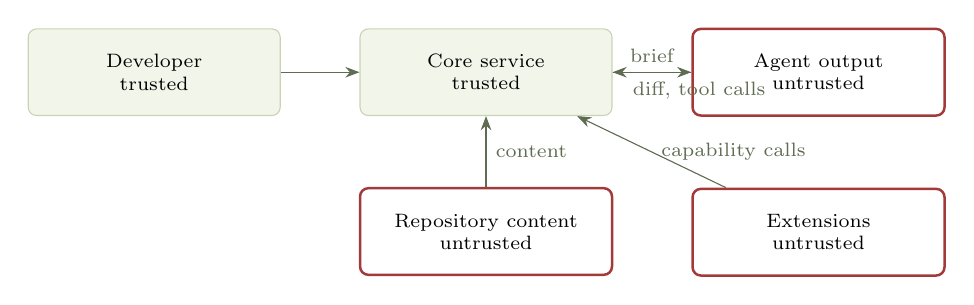
\begin{tikzpicture}[
  zone/.style={draw=xyraline,fill=xyrapanel,rounded corners=3pt,font=\scriptsize,align=center,minimum height=11mm},
  danger/.style={draw=xyrared,line width=0.9pt,fill=white,rounded corners=3pt,font=\scriptsize,align=center,minimum height=11mm},
  arr/.style={-{Stealth[length=1.8mm]},xyragrey,font=\scriptsize}
]
\node[zone,minimum width=32mm] (dev) {Developer\\trusted};
\node[zone,minimum width=32mm,right=10mm of dev] (core) {Core service\\trusted};
\node[danger,minimum width=32mm,right=10mm of core] (agent) {Agent output\\untrusted};
\node[danger,minimum width=32mm,below=9mm of agent] (ext) {Extensions\\untrusted};
\node[danger,minimum width=32mm,below=9mm of core] (repo) {Repository content\\untrusted};

\draw[arr] (dev) -- (core);
\draw[arr] (core) -- node[above] {brief} (agent);
\draw[arr] (agent) -- node[below,xshift=6mm] {diff, tool calls} (core);
\draw[arr] (ext) -- node[right] {capability calls} (core);
\draw[arr] (repo) -- node[right] {content} (core);
\end{tikzpicture}
\caption{Trust boundaries. Everything a model or a repository produces is untrusted input.}
\end{figure}

\subsection{Controls}

\begin{longtable}{@{}p{0.30\textwidth} p{0.62\textwidth}@{}}
\toprule
\textbf{Risk} & \textbf{Control} \\
\midrule
\endhead
Prompt injection from repository content & Repository text is data, never instruction. Tool calls originating from content patterns are rejected, and the Context Inspector shows provenance for every item \\
Secret exfiltration through context & Redaction runs before any content leaves the machine, covering keys, tokens, environment files and private keys, and the redaction is recorded \\
Malicious extension & Sandboxed execution with an explicit capability list, no ambient filesystem or network, and a trap disables the extension for the session \\
Destructive agent action & Write access is a property of the role, snapshots are used for execution, and every mutation is a reversible transaction with a commit boundary \\
Supply chain & Vendored dependencies at pinned revisions, license allow list enforced in continuous integration, signature verification on registry downloads \\
Credential handling & Provider credentials live in the platform keychain, are never written to the workspace, and are never included in context \\
Unbounded resource use & Every agent session and verification run carries a timeout, a token budget and a hard kill path \\
Data at rest & Workspace state is local. Nothing is uploaded without an explicit capability being enabled \\
\bottomrule
\caption{Security controls mapped to risks.}
\end{longtable}

\section{Privacy and telemetry}

Telemetry is off by default and is never a precondition for any feature. When a developer
enables it, the payload is enumerable in the settings surface before it is sent, contains no
source code, no file paths and no prompts, and can be inspected in a local log. Crash reports
are written locally and uploaded only on an explicit action.

\section{Accessibility}

Accessibility is an acceptance criterion on every interface issue rather than a milestone of
its own.

\begin{itemize}
  \item Every control has an accessible name and role, and every surface has a logical focus
  order.
  \item Every command is reachable from the keyboard, and the palette is the guaranteed path.
  \item Contrast meets the standard threshold in both themes, verified by an automated check
  in continuous integration.
  \item Severity is never conveyed by colour alone; it always carries a glyph and a word.
  \item Motion respects the platform reduced motion preference, including the activity pulse.
  \item Screen reader output is verified for the Mission Control and Verification Deck flows,
  because those are the surfaces that report autonomous work.
\end{itemize}

\section{Internationalisation}

Strings are externalised from the first commit, because retrofitting is expensive. The
initial shipping locales are English and Turkish. Locale affects interface strings only;
identifiers, log output and journal entries remain in English so that artefacts stay
portable across teams.

\section{Platform support}

\begin{table}[h]
\centering
\small
\begin{tabularx}{\textwidth}{l l X}
\toprule
\textbf{Platform} & \textbf{Status} & \textbf{Notes} \\
\midrule
macOS arm64 & Primary & Reference development and benchmark target \\
macOS x86\_64 & Supported & Built from the same source, verified in continuous integration \\
Linux x86\_64 & Supported & Distributed as a portable single file bundle \\
Linux arm64 & Best effort & Built, tested less frequently \\
Windows x86\_64 & Supported & Installer, path length and process semantics handled explicitly \\
\bottomrule
\end{tabularx}
\caption{Platform support matrix.}
\end{table}

\section{Packaging and updates}

\begin{itemize}
  \item Artefacts are produced by continuous integration from a clean checkout, never from a
  developer machine.
  \item Every artefact carries a checksum and, where the platform supports it, a signature.
  \item Updates are staged: a fraction of installations receive a release first, and a
  regression halts the rollout.
  \item An update never rewrites workspace state in place without a backup that the previous
  version can still read.
  \item An air gapped installation path exists, because enterprise customers require it and
  it also proves the build has no hidden network dependency.
\end{itemize}

\section{Risk register}

\begin{longtable}{@{}p{0.30\textwidth} p{0.14\textwidth} p{0.48\textwidth}@{}}
\toprule
\textbf{Risk} & \textbf{Severity} & \textbf{Mitigation} \\
\midrule
\endhead
Rendering framework churn upstream & Medium & Vendored and pinned, wrapped behind an internal crate so it can be replaced \\
Model provider terms change & High & Vendor routing is configurable per role, local models are a first class path, no feature depends on one provider \\
Autonomous run produces plausible but wrong work & High & Verification gate before display, adversarial review, one commit per ticket, journal, easy revert \\
Context engine underperforms naive stuffing & Medium & Permanent evaluation harness measuring first attempt success, with the naive strategy as the baseline \\
Scope creep into a general purpose editor & High & Non goals stated in Chapter one, every issue traceable to a story \\
Single maintainer bottleneck & High & Category partition designed for parallel work, documentation as the source of truth rather than tribal knowledge \\
Performance regression as features land & Medium & Budgets enforced by benchmark in continuous integration \\
Extension ecosystem security incident & Medium & Capability sandbox, signature verification, isolation on trap \\
License contamination through a transitive dependency & High & Allow list enforced mechanically on every build, vendored tree audited \\
\bottomrule
\caption{Risk register with mitigations that are implemented rather than aspirational.}
\end{longtable}

\chapter{Generation Prompts}
\label{ch:prompts}

This chapter turns the document into code. Each prompt is written to be pasted into an agent
session together with this document. They assume the agent can read files, run commands and
create commits, and they assume nothing else.

\section{Rules of engagement}

Prepend this to every session. It is the contract that keeps generated work consistent with
the specification.

\begin{lstlisting}
You are implementing Xyra, an agentic IDE, from a written specification.

The specification is authoritative. If your instinct disagrees with it, follow the
specification and state the disagreement in your final message rather than silently
deviating.

Rules that apply to every session:
1. Implement exactly one issue identifier from the register. Do not start another.
2. Never add a dependency whose license is outside MIT, Apache-2.0, BSD, ISC, Zlib,
   Unlicense or CC0. If you need one that is not, stop and report it.
3. Write no code comments. Names carry the meaning. Rationale goes in the commit body.
4. Never use an em dash anywhere: not in code, strings, documents or commit messages.
5. Interface copy is sentence case. No capitalised words.
6. Every control you add must already exist in the interface chapter. If it does not,
   stop and report the gap rather than inventing a control.
7. Every long running operation takes a budget and a cancellation token.
8. Write tests, including at least one for the failure path. Run them. Report the result
   with the exact command and its exit code.
9. Leave the working tree building and the test suite green. Do not commit; report the
   diff and let the supervisor commit.
10. Never run an interactive command or a process that does not exit. Use the
    non interactive flag, or start it detached and read the log.

When you finish, report: the issue identifier, the files changed, the test command and
its result, and anything in the specification you found ambiguous.
\end{lstlisting}

\section{Bootstrap prompt}

Run once, on an empty repository.

\begin{lstlisting}
Read the attached blueprint. Create the repository skeleton described in the architecture
chapter: a workspace manifest, one directory per crate listed in the crate topology table,
a lint and format configuration, a license allow list check, and a continuous integration
definition that runs format, lint, test and the license check.

Every crate is created with a doc header stating its single responsibility as written in
the crate topology table, and with a placeholder test so the suite is green from the first
commit. Do not implement behaviour yet.

This is issue PLA-001. Follow the rules of engagement.
\end{lstlisting}

\section{Category prompts}

Each of the twelve categories has a lead prompt that establishes shared understanding before
individual issues are executed against it.

\subsection{Platform}
\begin{lstlisting}
You own the PLA category: the window shell, the element toolkit, the core service and
the transport between them.

Read the architecture chapter and the design system section of the interface chapter.
Implement the design tokens exactly as tabulated: spacing, radius, control heights, text
sizes, icon sizes. No arbitrary values anywhere in the toolkit.

Then implement the controls listed in PLA-004 through PLA-012, each with its full state
set: default, hover, active, focused, disabled, loading. Every control gets an accessible
name and keyboard reachability. Every control gets an interface test through the harness.

Work issue by issue in the order given in the register. One issue, one report.
\end{lstlisting}

\subsection{Text core}
\begin{lstlisting}
You own the TXT category: the rope buffer and everything that edits it.

Correctness is the entire job here. Implement transactions such that undo restores both
content and selection, coalescing is predictable, and concurrent transactions on one buffer
are ordered rather than merged optimistically.

Write property tests before implementation: random edit sequences must round trip through
undo and redo, and the rope must agree with a naive string model on every operation.

Start with TXT-001 and proceed in register order.
\end{lstlisting}

\subsection{Syntax}
\begin{lstlisting}
You own the SYN category: parsing and everything derived from a parse tree.

The parse tree is the substrate for the context engine, not only for colouring. Symbol
extraction in SYN-008 must produce, for every file, the ordered symbol list with full
signatures, type declarations, documentation comments and outbound call edges, in the
shape the context chapter calls a Structural Context Protocol record.

Design that output format first, write golden tests for it against fixture files in each
supported language, then implement.
\end{lstlisting}

\subsection{Language}
\begin{lstlisting}
You own the LNG category: language server integration.

Supervision is as important as the features. A server that crashes restarts with backoff
and the editor never stops working. A server that lacks a capability degrades that feature
visibly rather than failing silently.

Implement LNG-001 and LNG-002 fully before any feature issue, because every feature depends
on correct capability negotiation.
\end{lstlisting}

\subsection{Project and version control}
\begin{lstlisting}
You own the PRJ category: the worktree, watching and git.

Two invariants: the developer's edit always wins over any automated change, and no
operation may leave the repository in a state the developer did not ask for. Every
destructive operation is reversible or confirmed.

Implement staging by hunk in PRJ-007 with the same data model the diff view uses, so the
two surfaces cannot disagree.
\end{lstlisting}

\subsection{Terminal}
\begin{lstlisting}
You own the TRM category: terminal emulation and process supervision.

TRM-007 is the issue that matters most: enforce the non interactive policy on commands
invoked by agents. A command that would prompt is refused with the correct non interactive
form stated, a process that does not exit is started detached with its log tailed, and a
command producing no output for a bounded period is terminated.

Implement TRM-001 and TRM-002 first, then TRM-007 before the remaining features.
\end{lstlisting}

\subsection{Context engine}
\begin{lstlisting}
You own the CTX category: the structural graph, the compression protocol, the budget
solver and the retrieval pipeline.

Read the context chapter completely before writing code. Implement in this order:
structural extraction, then the SCP record at three levels, then token counting with a
real tokeniser, then the budget solver, then delta encoding, then the assembly pipeline.
Similarity search comes last and is always labelled as a fallback in its results.

Build the evaluation harness described in CTX-040 early, not at the end. Every subsequent
change to the engine must be justified by a measured improvement in first attempt success,
compression ratio or escalation rate against the naive baseline.
\end{lstlisting}

\subsection{Agent layer}
\begin{lstlisting}
You own the AGT category: agent sessions, the tool surface and skills.

Every tool has a typed contract, a capability gate and an audit record. No tool grants
ambient authority. Write access is a property of the role as tabulated in the agent
chapter, not of the model.

AGT-017, the inactivity watchdog and hard kill path, is not optional and is not last. A
hung agent process must never be able to block the interface or a mission.
\end{lstlisting}

\subsection{Mission}
\begin{lstlisting}
You own the MIS category: the supervisor that runs a project to completion unattended.

The state machine is specified in the agent chapter. Implement it exactly, including the
four step failure escalation: retry, vendor swap, split with bounded depth, quarantine and
continue.

Two hazards to handle explicitly. The working tree reset between attempts must spare the
supervisor's own state directory, otherwise the supervisor destroys its own memory. And
ticket splitting must be depth bounded, otherwise a persistently failing ticket splits
forever.

State is written atomically after every transition. Prove resumption with a test that kills
the process mid ticket and continues.
\end{lstlisting}

\subsection{Verification}
\begin{lstlisting}
You own the VER category: everything that proves a change works.

Verification never touches the developer's working tree. Snapshot the change set into a
throwaway worktree and execute there.

Implement VER-001 through VER-003 first, because the mission category depends on them.
Then targeted test selection, then visual verification, then the adversarial sweep.

Every verdict is structured, with severity ranked issues, because verdicts feed automatic
fix loops rather than human reading.
\end{lstlisting}

\subsection{Fleet}
\begin{lstlisting}
You own the FLT category: multi repository operations.

Registration comes from the developer's provider, never from a hand written file. Impact
analysis must separate the repository that defines a contract from those that consume it,
because that ordering is what makes a cross repository change safe.

Each repository is verified independently before any linked change is prepared.
\end{lstlisting}

\subsection{Extensions}
\begin{lstlisting}
You own the EXT category: the extension host.

Extensions are untrusted. No ambient filesystem access, no network unless granted, an
explicit capability list in the manifest, and a trap disables the extension for the
session without affecting the editor.

Implement EXT-002 and EXT-010 before any contribution point, because isolation is the
feature.
\end{lstlisting}

\section{Issue prompt template}

For each issue in the register, substitute and run.

\begin{lstlisting}
Implement issue {ID}: {title}.

Read these sections of the blueprint before writing code:
- the architecture chapter section for {crate}
- the interface chapter section for {surface}, if this issue touches the interface
- the user stories that reference this capability: {story ids}

Acceptance:
- The behaviour matches the specification exactly.
- Tests exist including a failure path test, and they pass.
- No control exists that is not specified in the interface chapter.
- No dependency was added outside the license allow list.
- The operation has a budget and a cancellation path if it can run long.
- Accessible name and keyboard reachability exist for every new control.

Dependencies already landed: {depends}.
Follow the rules of engagement. Report when done.
\end{lstlisting}

\section{Self hosting prompt}

The most efficient way to build Xyra is to use the existing Xyra mission supervisor to build
it. Once the register is loaded as a ticket graph, the loop in the agent chapter applies to
this project as it does to any other.

\begin{lstlisting}
Convert the issue register in the blueprint into a mission ticket graph. Each issue becomes
one ticket: the identifier is the ticket identifier, the issue text is the scope, and the
Depends column becomes the dependency list.

Then run the mission to completion with these budgets: attempts per ticket three, split
depth one, and a stop on five consecutive failures.

For every ticket, the brief is the issue prompt template filled in from the register, with
the rules of engagement prepended.

Verification for this project is the workspace test suite plus the format and lint checks
plus the license allow list check. A ticket counts as done only when all four pass in an
isolated snapshot.
\end{lstlisting}

\section{Review prompt}

Run against every diff before it is accepted, ideally on a different vendor from the one that
wrote it.

\begin{lstlisting}
You are reviewing a diff produced by another vendor against a written specification.

Check, in this order:
1. Correctness. Does it do what the issue says, including the failure path.
2. Specification fidelity. Does any control, message or behaviour deviate from the
   blueprint. Quote the deviation.
3. Boundaries. Does it call across a layer in the wrong direction, or reach into another
   category's crate.
4. Security. Untrusted input treated as instruction, secrets in context, missing capability
   gate, unbounded resource use.
5. Conventions. Comments present, em dashes present, capitalised interface copy, arbitrary
   spacing values instead of tokens.

Return a structured verdict: severity per finding, file and line, and a blocking decision.
Default to blocking when uncertain about correctness or security.
\end{lstlisting}

\section{Specification amendment prompt}

The document is the source of truth, which means it must be maintained as the code teaches
you things.

\begin{lstlisting}
While implementing {ID} you found that the blueprint is wrong, ambiguous or incomplete.

Do not silently deviate. Produce an amendment:
- The exact section and sentence that is wrong.
- What the code must do instead, and why the specification could not have anticipated it.
- Any other section that must change for the document to stay internally consistent.
- The stories and issues affected.

Emit the amendment as a patch to the blueprint source alongside the code change. The
document and the code land together or not at all.
\end{lstlisting}

\appendix

\chapter{Traceability}
\label{ch:traceability}

This chapter exists to keep the document honest. Every surface must be justified by a story,
every story must be delivered by issues, and every issue must belong to a category with an
owner. A row that cannot be completed is a defect in the specification, not a detail to be
resolved later.

\section{Story to issue to surface}

\begin{longtable}{@{}p{0.07\textwidth} p{0.30\textwidth} p{0.36\textwidth} p{0.21\textwidth}@{}}
\toprule
\textbf{Story} & \textbf{Capability} & \textbf{Delivered by} & \textbf{Surface} \\
\midrule
\endhead
S-01 & Orient in an unknown repository & CTX-008, CTX-010, FLT-007 & Atlas \\
S-02 & Blast radius before a change & CTX-009, LNG-012, AGT-007 & Workbench, Atlas \\
S-03 & History behind a line & PRJ-011, CTX-030 & Workbench, Inspector \\
S-04 & Trust a small change & VER-002, VER-003, MIS-006 & Workbench, Deck \\
S-05 & Concurrent human edit & AGT-024, AGT-025 & Workbench \\
S-06 & Adversarial review & AGT-026, AGT-027, AGT-028 & Deck, Theatre \\
S-07 & Unattended feature delivery & MIS-002 to MIS-007, MIS-020 & Mission Control \\
S-08 & Failure without stopping & MIS-008 to MIS-011 & Mission Control \\
S-09 & Survive a closed laptop & MIS-001, MIS-018 & Mission Control \\
S-10 & Stop cleanly & MIS-015 & Mission Control, title bar \\
S-11 & Cap the cost & MIS-013 & Mission Control, status bar \\
S-12 & Visual correctness & VER-006, VER-007 & Deck \\
S-13 & Match a design & VER-007, AGT-011 & Deck, Mission Control \\
S-14 & Cross repository contract change & FLT-004, FLT-005, FLT-006 & Atlas, Mission Control \\
S-15 & Register a fleet & FLT-001, FLT-002 & Atlas, first run \\
S-16 & See what the agent reads & CTX-020, CTX-028, CTX-038 & Inspector \\
S-17 & Redirect attention & CTX-027, CTX-038 & Inspector \\
S-18 & Decide a fork deliberately & MIS-016, AGT-015 & Decision cards \\
S-19 & Branch from a past decision & MIS-014, PRJ-015 & Atlas history \\
S-20 & Enforce standards mechanically & AGT-020, AGT-021, AGT-027 & Inspector, Deck \\
S-21 & Prove what happened & MIS-014, AGT-030, VER-015 & Deck, journal \\
S-22 & Control what leaves the machine & CTX-038, CTX-039 & Inspector, settings \\
S-23 & Agent hang cannot break the editor & AGT-017, PLA-016 & All \\
S-24 & No interactive command hangs & TRM-007, TRM-008, AGT-022 & Terminal, Theatre \\
S-25 & Work while a mission runs & VER-002, VER-005, AGT-025 & Workbench, Mission Control \\
\bottomrule
\caption{Every story maps to issues and to the surfaces that expose it.}
\end{longtable}

\section{Surface to category ownership}

\begin{table}[h]
\centering
\small
\begin{tabularx}{\textwidth}{l l X}
\toprule
\textbf{Surface} & \textbf{Owning category} & \textbf{Contributing categories} \\
\midrule
Workbench & TXT & SYN, LNG, PRJ, AGT, PLA \\
Mission Control & MIS & AGT, VER, PLA \\
Agent Theatre & AGT & MIS, PLA \\
Context Inspector & CTX & AGT, PLA \\
Verification Deck & VER & MIS, PLA \\
Atlas & CTX & PRJ, FLT, PLA \\
Terminal, inside Workbench & TRM & PLA \\
Settings and palette & PLA & all \\
\bottomrule
\end{tabularx}
\caption{Surface ownership. One category owns each surface and is accountable for it.}
\end{table}

\chapter{Formats and Glossary}

\section{Workspace state layout}

\begin{lstlisting}
.xyra/
  mission.json        durable mission state, atomically replaced
  mission.log         supervisor log, append only
  journal.jsonl       decisions anchored to commits
  fleet.json          registered repositories and roles
  policy.toml         verification and review policy for this repository
  settings.toml       workspace settings, layered over user settings
  skills/             workspace skills, highest precedence
  index/              symbol table, import graph, chunk metadata
  vectors/            quantised embeddings, memory mapped
  cache/              content addressed artefacts, safe to delete
  views/              generated report artefacts
\end{lstlisting}

Deleting the entire directory must degrade the product to a cold start and must never
corrupt the repository. This is a tested invariant, not an intention.

\section{Ticket schema}

\begin{lstlisting}
{
  "id": "MIS-007",
  "title": "Commit per verified ticket",
  "scope": "precise enough to act on without asking a question",
  "files": ["crates/xyra-mission/src/commit.rs"],
  "depends_on": ["MIS-006"],
  "status": "pending | ready | running | verifying | done | retry | split | quarantined | skipped",
  "depth": 0,
  "attempts": 0,
  "vendor_index": 0,
  "commit": null,
  "notes": []
}
\end{lstlisting}

\section{Verification verdict schema}

\begin{lstlisting}
{
  "ok": true,
  "command": "cargo test --workspace",
  "exit_code": 0,
  "duration_ms": 41230,
  "scope": "targeted | full",
  "failures": [],
  "output_tail": "...",
  "snapshot": "throwaway worktree identifier"
}
\end{lstlisting}

\section{Review verdict schema}

\begin{lstlisting}
{
  "decision": "clean | approve_with_notes | block | inconclusive",
  "lenses": ["correctness", "security", "conventions"],
  "findings": [
    {
      "severity": "critical | high | medium | low",
      "lens": "security",
      "file": "crates/xyra-agent/src/tools.rs",
      "line": 214,
      "issue": "one sentence statement of the defect",
      "evidence": "concrete inputs or state that produce it"
    }
  ],
  "policy": "path rule that decided the blocking threshold"
}
\end{lstlisting}

\section{Glossary}

\begin{longtable}{@{}p{0.26\textwidth} p{0.66\textwidth}@{}}
\toprule
\textbf{Term} & \textbf{Definition} \\
\midrule
\endhead
Accelerator & A mechanism that reduces latency or repeated work without changing which context items are selected \\
Agent range & A contiguous region of a buffer written by an agent and not yet accepted by a human \\
Atlas & The structural surface: topology, impact, ownership and history \\
Budget solver & The component that selects context items under a token limit using value, cost, redundancy and dependency \\
Capability & An explicitly granted permission for an integration, tool or extension \\
Council & Adversarial review of a diff by a rival vendor across parallel lenses \\
Delta encoding & Transmitting only what changed since the previous session, referencing the rest by handle \\
Escalation rate & The frequency with which an agent must request a higher context tier \\
Fleet & A registered group of repositories treated as one unit for search, impact and execution \\
Handle & A content addressed reference to a body that can be expanded on request \\
Impact closure & The deterministic set of files affected by a change, by transitive distance \\
Intent & A user action sent from a surface to the core, never a direct mutation \\
Journal & The append only record of decisions anchored to commits \\
Lens & One perspective in a review: correctness, security or conventions \\
Mission & An objective decomposed into a ticket graph and executed to completion \\
Projection & A serialisable snapshot of state prepared for one surface to render \\
Quarantine & The state of a ticket that exhausted its failure policy and needs a human \\
Role & An agent specialisation with its own mandate, tool grant and write access \\
SCP & Structural Context Protocol, the compressed structural representation of a file \\
Skill & A durable instruction set injected into agent sessions, resolved by precedence \\
Snapshot & A throwaway worktree containing a change set, used for verification \\
Surface & One of the six primary product views \\
Ticket & The unit of autonomous work: one session, one verification, one commit \\
Tier & A level on the context ladder, from repository skeleton to runtime evidence \\
\bottomrule
\caption{Glossary of terms used consistently throughout this document.}
\end{longtable}

\section{Document maintenance}

This document is the source of truth for the product. Three rules keep it that way.

\begin{enumerate}
  \item Code that contradicts the document is a defect in one of them, and the discrepancy
  is resolved before the code lands, not afterwards.
  \item An amendment lands in the same change as the code it describes, using the amendment
  prompt in Chapter~\ref{ch:prompts}.
  \item A new surface, control or capability enters through a story first. If no persona
  needs it, it does not ship.
\end{enumerate}


\end{document}
